\chapter{Feldman--Cousins 方法详述}
%=====================================================================

在精确测量中微子振荡参数的过程中，置信区间的构造方式直接影响物理结论的可靠性。对于大统计量情形，基于极大似然比的检验统计量通常满足 Wilks 定理的渐近条件，其 $\Delta\chi^2$ 分布可近似为自由度等于待测参数个数的卡方分布，从而可以使用固定的阈值（例如一维情形下 $\Delta\chi^2=1$ 对应 $1\sigma$）来构造置信区间\cite{Wilks:1938dza}。然而，在统计量有限或似然函数结构复杂的情况下，Wilks 定理所依赖的正则性条件可能被破坏，此时若仍然沿用渐近阈值，可能导致置信区间覆盖率偏离名义置信度。特别是在 $\Delta m^2_{31}$ 的测量问题中，JUNO 实验在低统计量阶段（例如 50 天统计量）所得到的轮廓 $\chi^2$ 曲线往往呈现明显的非二次形态，并伴随多个局部极小值。这些“bad minima”来源于统计涨落以及振荡相位简并结构，使得基于单次数据集的点估计可能远离真实注入值，甚至产生多个不连续的置信区间。

Asimov 数据集假设观测结果严格等于理论期望值，因此只能反映理想化的平均灵敏度，无法体现真实实验中统计涨落所引起的多重极小值和非高斯行为。在这种情况下，单纯依赖 Asimov 灵敏度或渐近公式并不足以保证统计结论的稳健性。为了真实研究统计波动对置信区间结构与覆盖率的影响，有必要通过大量包含随机涨落的 Toy Monte Carlo 伪实验来构造检验统计量的经验分布，从而直接检验覆盖性质。Feldman–Cousins（FC）方法\cite{Feldman_1998}正是建立在这一思想之上：通过在给定假设参数点下生成大量伪实验，并对每个伪实验重复完整拟合流程，构造 $\Delta\chi^2$ 的经验分布，再从该分布中提取满足给定置信水平的临界值\cite{Acero2022ProfiledFC}。与 Wilks 定理不同，FC 方法不依赖渐近近似，因此在低统计量或似然函数高度非线性的情况下仍能保证正确的频率学覆盖率。

本章的核心目标是在 JUNO 早期运行条件下系统评估各振荡参数的覆盖行为，并明确在何种情况下可以安全使用 Wilks 近似，何种情况下必须采用 Feldman–Cousins 构造。通过系统的伪实验研究，我们发现：在 50 天统计量下，太阳振荡区参数 $\Delta m^2_{21}$ 与 $\sin^2\theta_{12}$ 的 $\Delta\chi^2$ 行为与自由度为 2 的卡方分布相符，Wilks 近似在测试区间内成立，因此可以使用常规定义的 $\Delta\chi^2$ 阈值构造置信域；而对于 $\Delta m^2_{31}$，由于似然面存在明显的多重局部极小值与非抛物线结构，其 $\Delta\chi^2$ 分布显著偏离 Wilks 预期，一维情形下的经验临界值明显大于 1。因此，在该统计量条件下必须采用 Feldman–Cousins 方法以保证正确覆盖率。基于 FC 构造得到的 $\Delta m^2_{31}$ 相对精度约为 $1.4\%$（50 天曝光），略差于当前全球拟合结果（约 $1.1\%$）。这一结果为 JUNO 合作组在首篇物理结果文章中暂不直接给出 $\Delta m^2_{31}$ 精确测量值提供了统计依据，该建议最终被合作组采纳。

本章首先分析 Asimov 灵敏度方法在低统计量情形下的局限性，随后回顾 Wilks 定理的适用条件及其在本问题中的失效原因；在此基础上系统介绍 Feldman–Cousins 方法的基本思想与实现流程，并通过覆盖率研究分别对 $\Delta m^2_{21}$、$\sin^2\theta_{12}$ 和 $\Delta m^2_{31}$ 进行一维或二维 FC 构造。最后，我们讨论 FC 临界值对 $\Delta m^2_{31}$ 扫描区间选择的依赖性，说明在存在多个局部极小值时必须采用足够宽的参数扫描范围和多起始点拟合策略，以避免遗漏全局最优解并确保置信区间具有正确的覆盖性质。


\section{Asimov 灵敏度的局限性}
\label{sec:asimov_limitation}

在研究低统计量下拟合与置信区间构造的行为时，需要注意 Asimov 数据集的局限性。Asimov 数据集只反映了理想条件下，无统计偏差下的期望结果，不包含实际观测中的统计扰动。因此，基于 Asimov 的灵敏度评估只给出了理论上的置信区间估计，并未涵盖统计涨落导致的分布非高斯性和偏离情形。其常常给出光滑且单峰的 $\Delta \chi^2$ 侧向轮廓化曲线，从而暗示单一连续的置信区间。但真实观测中存在统计涨落和系统误差波动，这些随机效应会显著改变轮廓形状并产生多重局部极小值。特别是当参数估计过程存在不稳定性或对 $\chi^2$ 响应非线性时（例如多峰或参数边界问题），Asimov 预测可能会严重失真，使得实际覆盖率与名义覆盖率不符。

\begin{figure}[htbp]
  \centering
  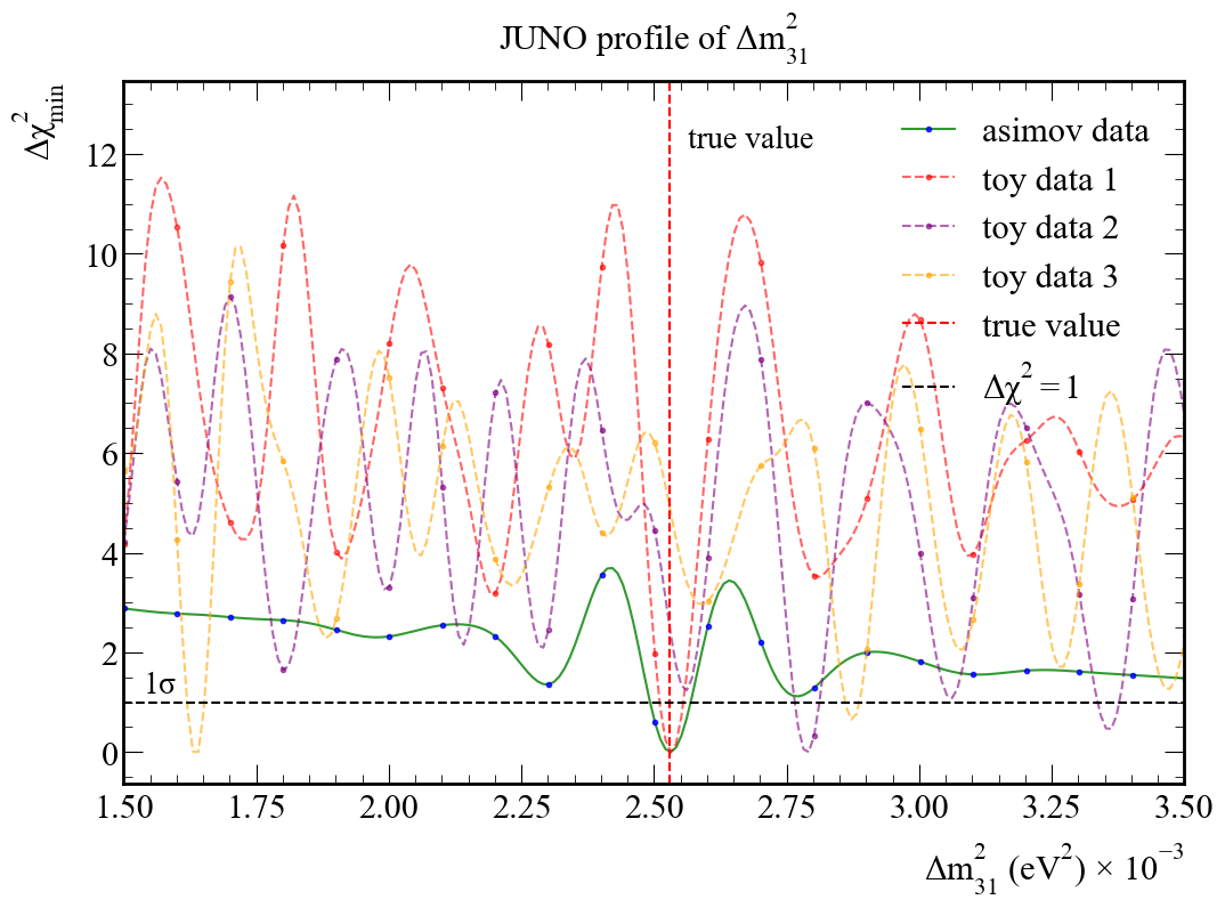
\includegraphics[width=0.9\linewidth]{Img/asimov-data.png}
  \bicaption[$\Delta m^2_{31}$ 的 $\Delta\chi^2$ 轮廓（Asimov 与若干 toy 实验，30 天统计量）]{$\Delta m^2_{31}$ 的 $\Delta\chi^2$ 轮廓（Asimov 与若干 toy 实验，30 天统计量）。绿色实线为 Asimov 数据得到的 $\Delta\chi^2$ 轮廓，显示出靠近真值（红色虚线）处的单一平滑极小值；按 Wilks 近似，这会对应单一连续的 $1\sigma$ 区间（图中黑色虚线为 $\Delta\chi^2 = 1$）。彩色虚线为三个独立 toy-MC 样本的轮廓（包含统计与系统误差波动）。可以看到实际涨落会显著改变轮廓形状：toy 曲线出现许多明显的局部极小值。有些局部极小值比 Asimov 情形更深并且偏离名义真值。这种多峰/多极小值行为会使得使用固定 $\Delta\chi^2$ 截值（Wilks 截断）得到的不一定是连续区间，可能出现不相交的置信域。}{Profile $\Delta\chi^2$ of $\Delta m^2_{31}$ for Asimov and several toy experiments (30 days exposure). The green curve is the Asimov (median) $\Delta\chi^2$ profile, which shows a single, relatively smooth minimum near the true value (red dashed vertical line) and would---under Wilks' approximation---suggest a single continuous $1\sigma$ interval (black dashed horizontal line at $\Delta\chi^2 = 1$). The colored dashed curves are $\Delta\chi^2$ profiles from three independent toy Monte-Carlo realizations (statistical and systematics fluctuations included). Real-data fluctuations substantially distort the profile: toy profiles exhibit many pronounced local minima, some of which are much deeper than nearby Asimov values and lie away from the nominal true value. Such behaviour can produce multiple disjoint confidence regions when one uses fixed $\Delta\chi^2$ thresholds (Wilks cuts).}
  \label{fig:asimov_dm31_profile}
\end{figure}

图~\ref{fig:asimov_dm31_profile} 给出了 30 天统计量下 $\Delta m^2_{31}$ 的实例：绿色曲线是 Asimov 轮廓，呈现单一平滑极小值；而多条彩色虚线（不同 toy-MC 实现）则展现出许多更深或位置不同的局部极小值。实际涨落常使某些局部极小值变得更低且更靠近数据所偏向的值，结果在应用固定 $\Delta\chi^2$ 截断（例如 $\Delta\chi^2 = 1$ 的 1$\sigma$ 判据）时可能得到多个不相交的置信区间或错误的覆盖概率。综上所述，Asimov-based 的灵敏度估计在低统计、参数空间非线性或存在多重解的情形下容易误导决策；因此必须通过大量 toy-MC 生成检验统计量的经验分布（例如采用 Feldman–Cousins 方法）来确定参数相关的临界 $\Delta\chi^2$，从而保证置信区间的频率学覆盖性质。

\begin{figure}[htbp]
  \centering
  \begin{subfigure}[t]{0.48\textwidth}
    \centering
    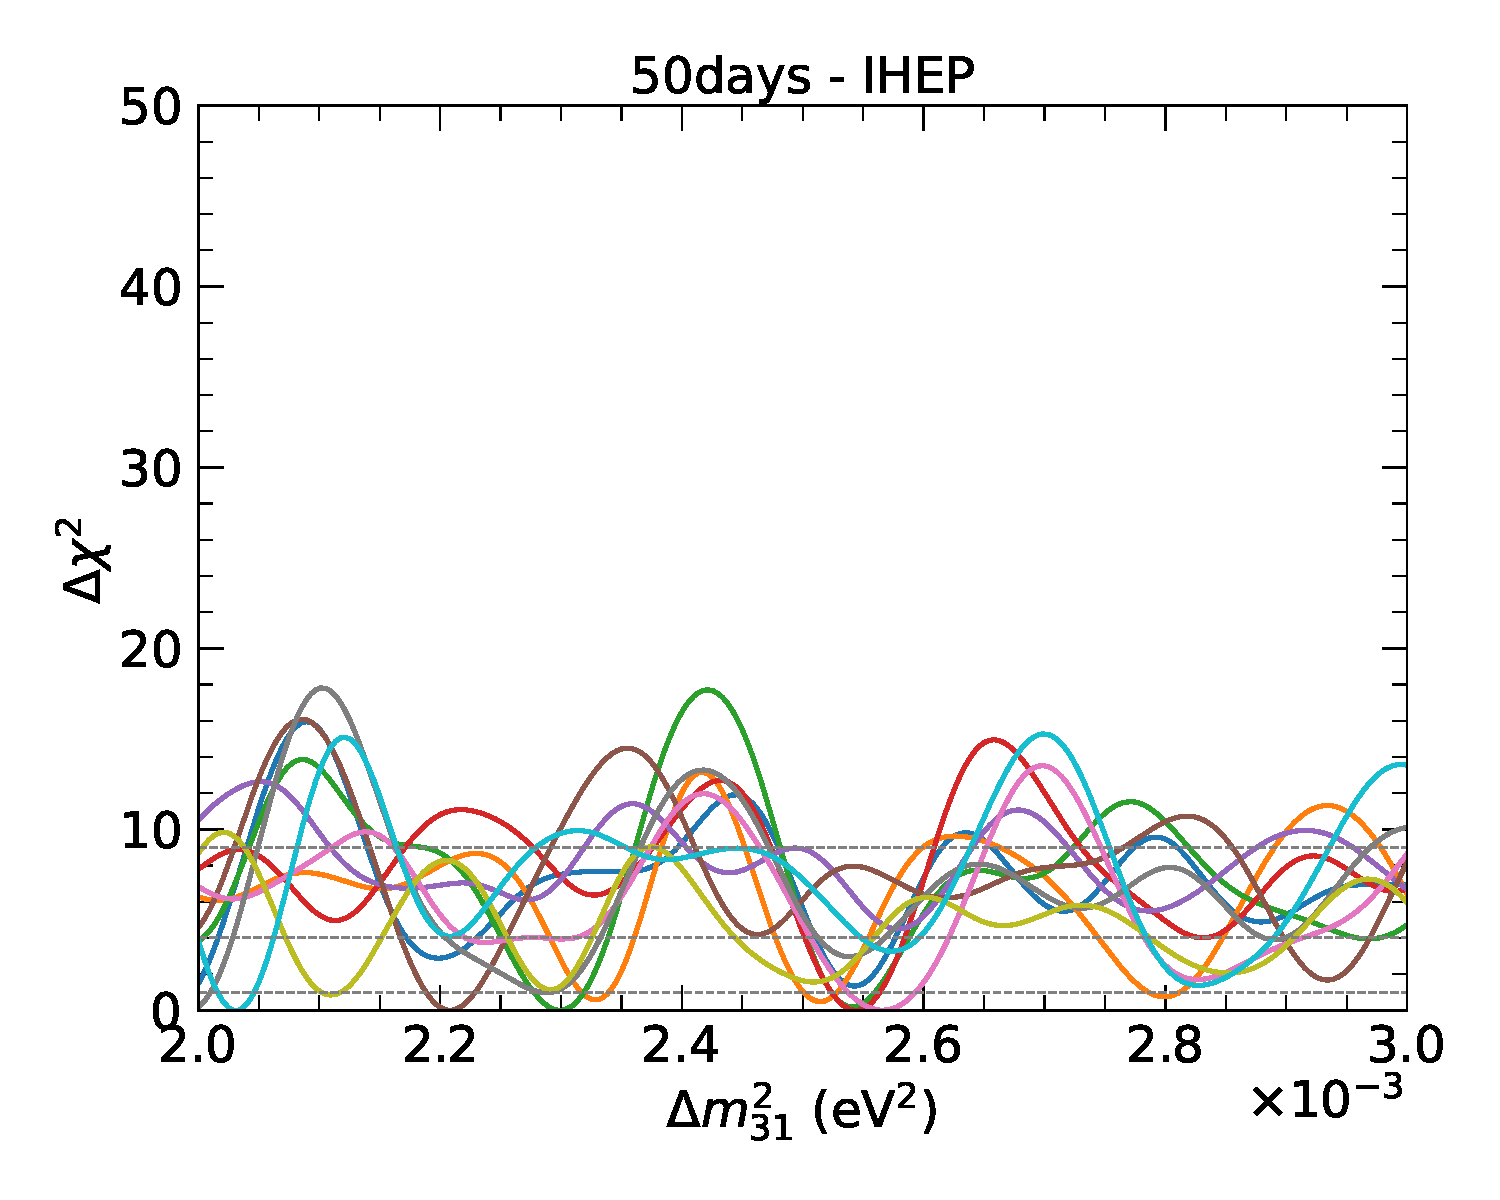
\includegraphics[width=\linewidth]{Img/Jingqin_50days_dmsq31_profile.pdf}
    \caption{50 天统计量}
    \label{fig:dm31_profile_50days}
  \end{subfigure}
  \hfill
  \begin{subfigure}[t]{0.48\textwidth}
    \centering
    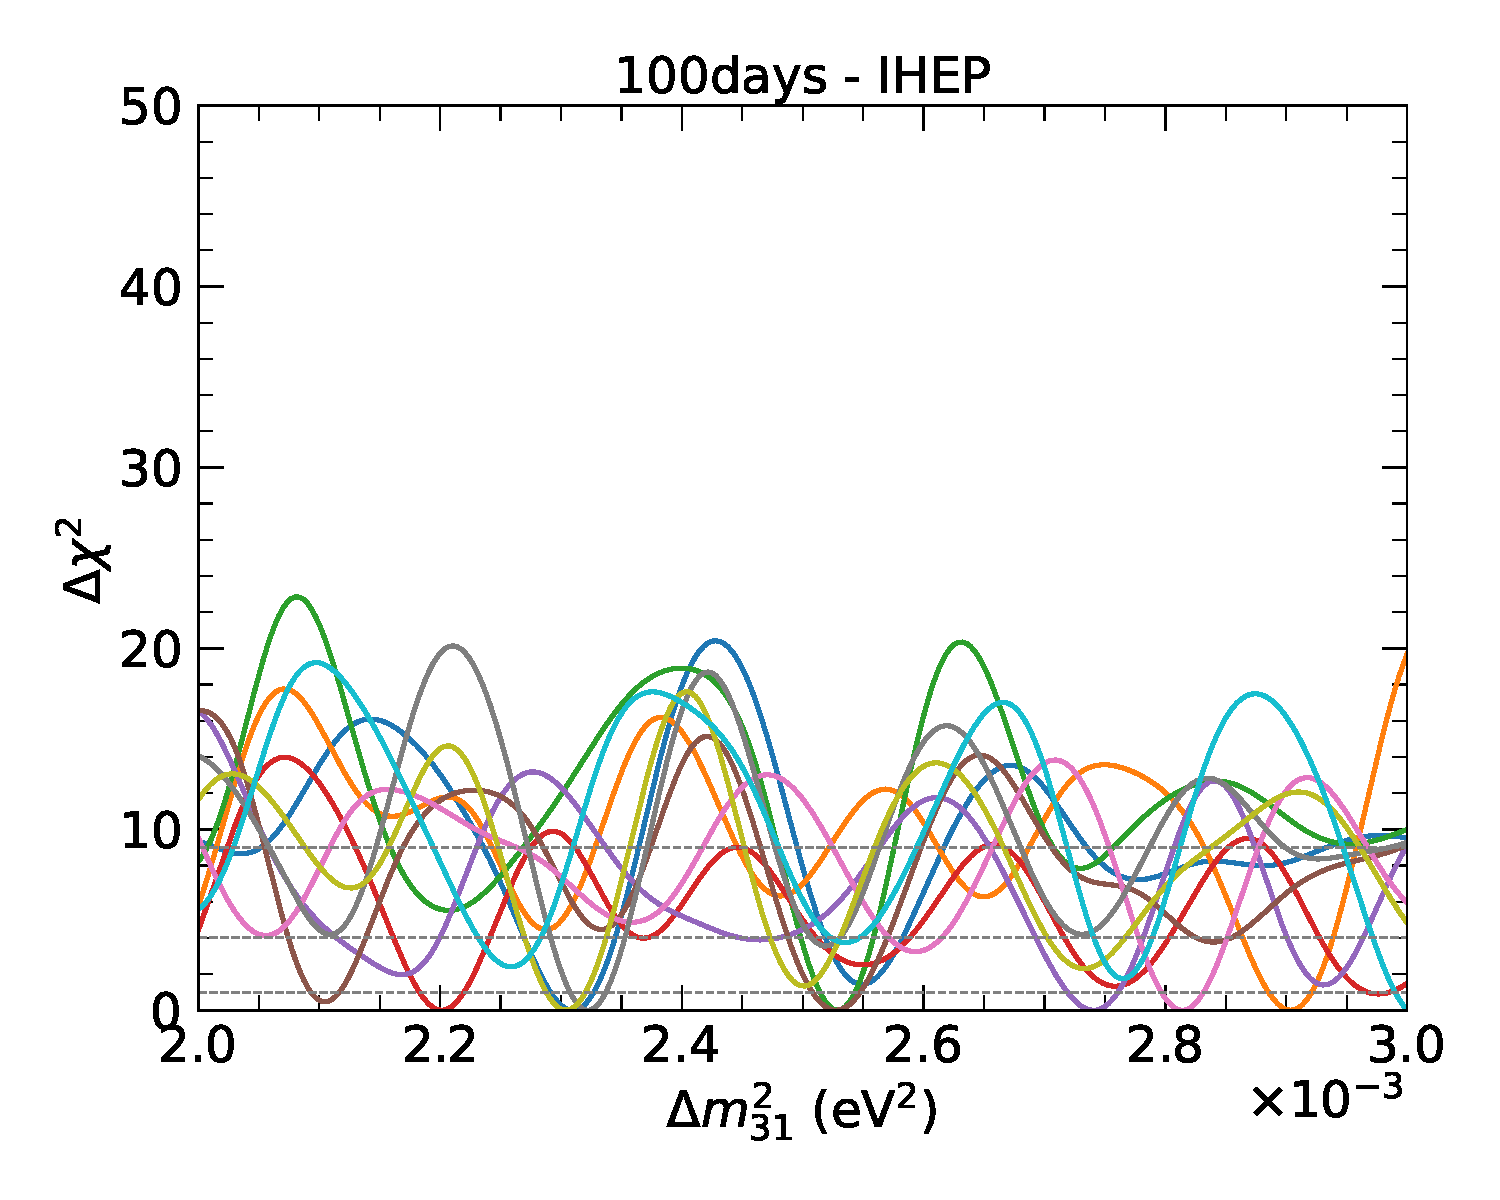
\includegraphics[width=\linewidth]{Img/Jingqin_100days_dmsq31_profile.pdf}
    \caption{100 天统计量}
    \label{fig:dm31_profile_100days}
  \end{subfigure}

  \vspace{0.4em}

  \begin{subfigure}[t]{0.48\textwidth}
    \centering
    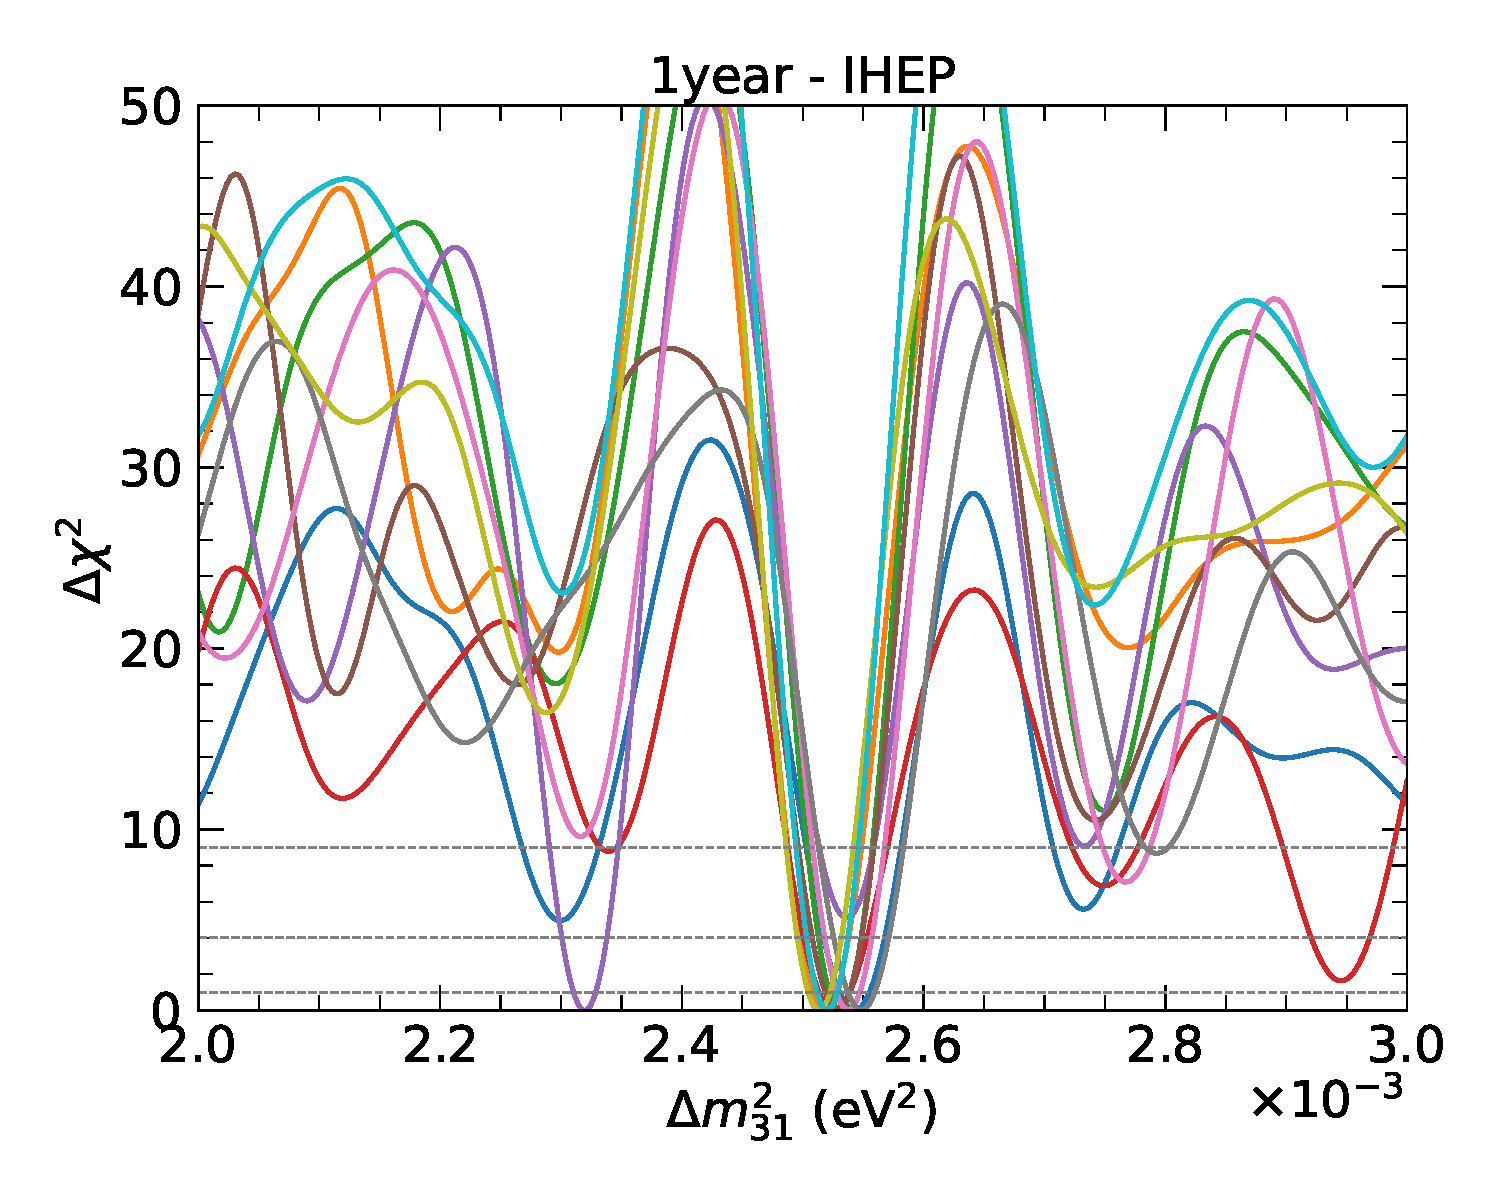
\includegraphics[width=\linewidth]{Img/Jingqin_1years_dmsq31_profile.pdf}
    \caption{1 年统计量}
    \label{fig:dm31_profile_1year}
  \end{subfigure}
  \hfill
  \begin{subfigure}[t]{0.48\textwidth}
    \centering
    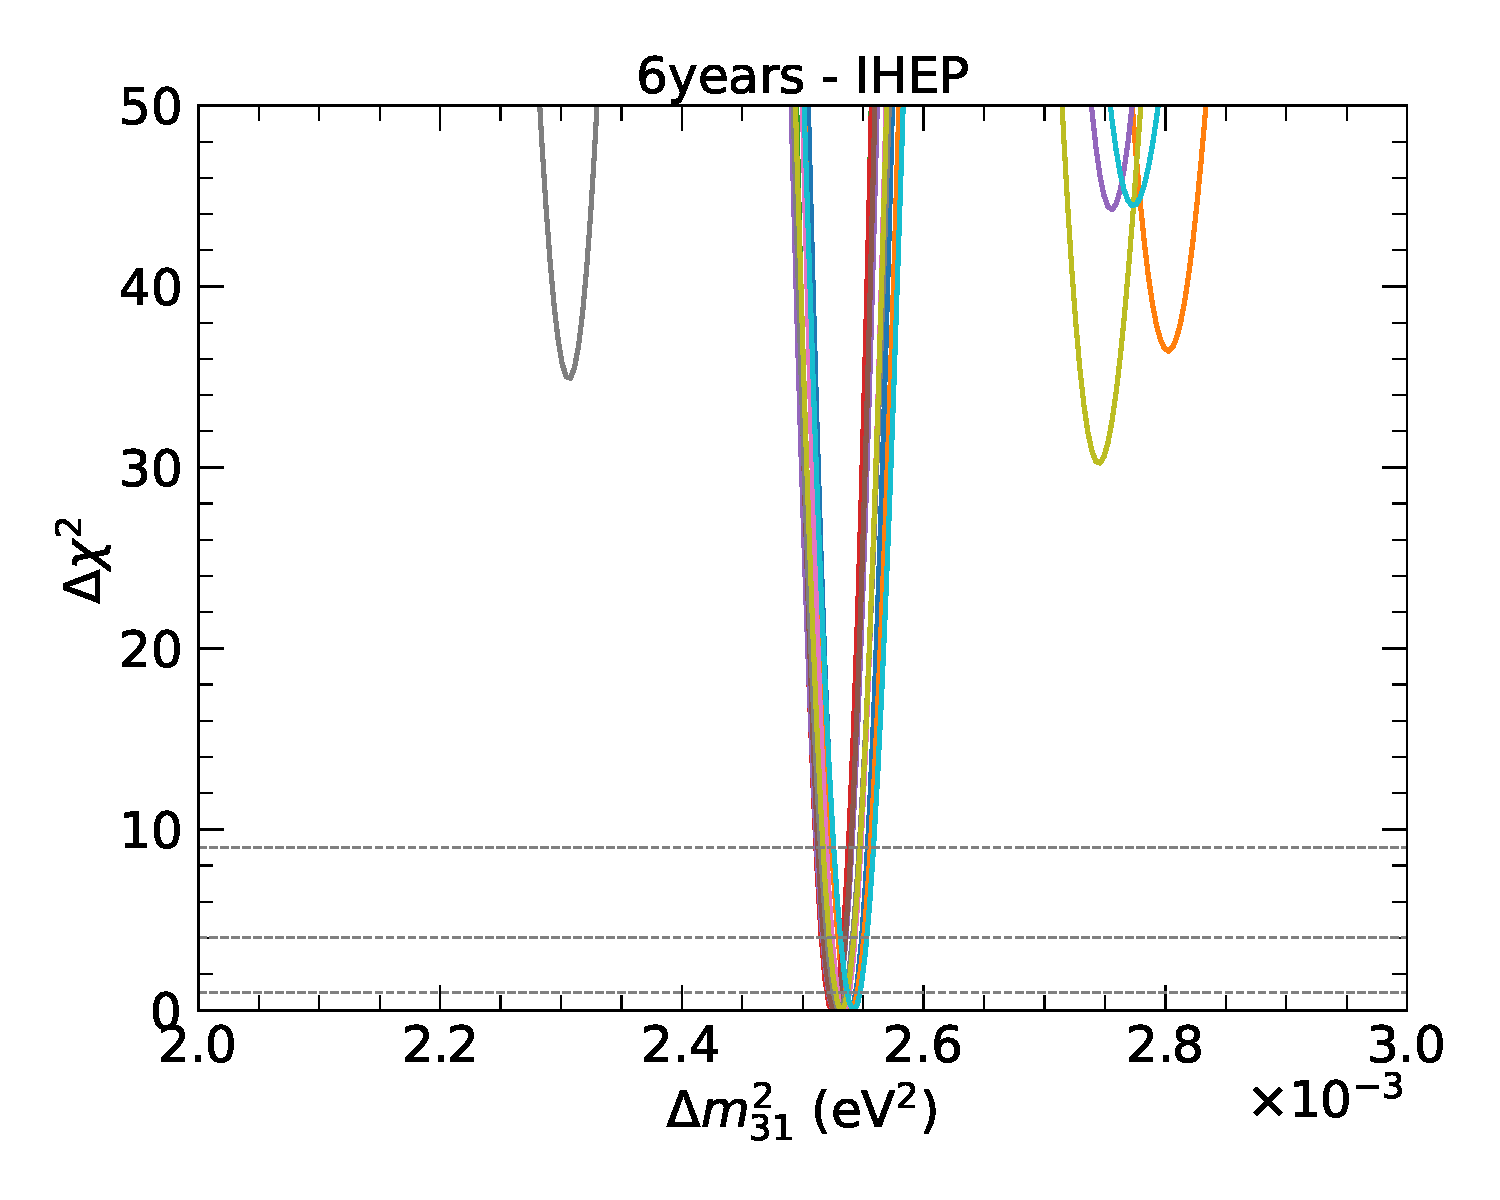
\includegraphics[width=\linewidth]{Img/Jingqin_6years_dmsq31_profile.pdf}
    \caption{6 年统计量}
    \label{fig:dm31_profile_6years}
  \end{subfigure}

  \bicaption[四种统计量下的 $\Delta m^2_{31}$ 侧向轮廓化曲线]{四种统计量下的 $\Delta m^2_{31}$ 侧向轮廓化曲线。}{Profile $\Delta\chi^2$ curves of $\Delta m^2_{31}$ for four different exposures. }
  \label{fig:dm31_profile_exposure}
\end{figure}

图~\ref{fig:dm31_profile_exposure} 展示了四种不同统计量下的 $\Delta m^2_{31}$ 的 $\Delta\chi^2$ 轮廓，可以看到，随着统计量增加，局域极小值和不连续区间出现的概率降低，轮廓趋于单峰和平滑。

\section{Wilks 定理的适用条件与局限}
\label{sec:wilks_limit}

Wilks 定理为基于对数似然比的检验提供了一种构造置信区间的渐近近似方法。设 $\delta$ 为感兴趣的物理参数，$\boldsymbol{\eta}$ 为冗余参数（nuisance parameters），定义检验统计量为：

\begin{equation}
\lambda_i \;=\; -2\ln\frac{\mathcal{L}(\boldsymbol{x}\mid\delta_i,\hat{\hat{\boldsymbol{\eta}}})}{\mathcal{L}(\boldsymbol{x}\mid\hat\delta,\hat{\boldsymbol{\eta}})}\,,
\end{equation}

其中，分子是在给定参数值 $\delta=\delta_i$ 的条件下，对冗余参数进行最大化所得的条件最大似然值（以双帽号标注）；分母则是对所有参数同时进行最大化得到的全局最大似然值（以单帽号标注）。Wilks 定理指出：在满足特定“正则性条件”的前提下，当样本量趋于无穷大时，上述统计量渐近服从自由度等于待测参数个数的卡方分布。因此，可直接采用卡方分布的分位数作为界定置信区间的阈值（例如，在 1 自由度下，$\lambda=1, 4, 9$ 分别对应约 68.27\%、95.45\% 与 99.73\% 的置信水平）\cite{Wilks:1938dza}。

然而，Wilks 近似的成立依赖于一系列关键假设 \cite{Wilks:1938dza, Fan:2000gm, Cranmer:2005hi, Cowan:2010js, ParticleDataGroup:2024cfk}，主要可归纳为以下三点：

\begin{itemize}[leftmargin=*,nosep]
  \item \textbf{嵌套假设（Nested hypotheses）}：被检验的零假设必须是备择假设的一个特例。在参数估计问题中，检验“参数等于某一特定值”通常满足此条件。
  \item \textbf{似然函数的光滑性（Smoothness of the likelihood）}：对数似然函数在真实参数附近须足够光滑，可用二阶泰勒展开近似（即呈现抛物线特征）。同时，参数必须严格位于定义域内部，且最大似然估计值在局部是唯一的。这保证了估计量的渐近正态性与似然比统计量的卡方行为。
  \item \textbf{大样本极限（Asymptotic limit）}：样本量需足够大，以确保上述渐近展开有效，并使高阶项的贡献可以忽略不计。
\end{itemize}

在实际物理分析中，若上述任一假设遭到破坏，Wilks 近似便可能失效。导致其失效的常见情形包括：真实参数靠近或位于物理边界（boundary）、复杂的参数映射导致似然面呈现强烈的非二次型特征、似然空间存在多个分离的局部极小值（multi-modal likelihood），或是样本量过小导致高阶项不可忽略等 \cite{Cowan:2010js, Cranmer:2005hi}。在这些非正则情形下，若强行采用 Wilks 定理给出的固定 $\Delta\chi^2$ 阈值，将会得出错误的置信区间，最典型的表现为\textbf{实际覆盖率（coverage probability）偏离名义置信水平}（例如出现“欠覆盖”现象，即区间包含真值的真实概率低于声称的置信度）。

在 JUNO 实验的早期运行阶段（低曝光量、低统计量），对 $\Delta m^2_{31}$ 的测量恰好打破了上述部分正则性条件。具体而言，通过轮廓似然方法（profile likelihood）提取的 $\Delta\chi^2$ 曲线在 $\Delta m^2_{31}$ 方向上显著偏离抛物线形状，且往往伴随多个明显的局部极小值（详见第~\ref{fig:dm31_profile_exposure}节的轮廓图），这直接违背了局部椭球近似的前提。其后果是，若遵循 Wilks 近似采用 $\Delta\chi^2=1$ 作为 $1\sigma$ 的临界值，将严重低估实际所需的阈值，导致对 $\Delta m^2_{31}$ 构造的置信区间出现\textbf{欠覆盖}。在我们的模拟覆盖性测试中（详见第~\ref{sec:FC_coverage}节），基于数据实证提取的一维经验临界值约为 $\Delta\chi^2_{\mathrm{crit}}\approx1.57$，显著高于 Wilks 近似的 1.0，这为 Wilks 定理在该场景下的失效提供了直接的定量证据。

综上所述，当面临此类非正则情况时，应摒弃单纯依赖 Wilks 近似的固定阈值法，转而采用基于伪实验（Toy Monte Carlo）的数据驱动方法（如 Feldman--Cousins 构造法）。通过这种方法，可针对每一个假设的参数点计算出具有参数依赖性的临界 $\Delta\chi^2$ 值，从而从根本上保证所构造置信区间的频率学覆盖性质严格达标（详见第~\ref{sec:FC_coverage}节）\cite{Feldman_1998, Cranmer:2005hi}。


\section{Feldman--Cousins 方法的核心思想}
\label{sec:FC}

针对 Wilks 定理在非正则情形下的局限性，Feldman 与 Cousins 提出了一种基于似然比排序原则（Likelihood Ratio ordering principle）构造置信区间的方法 \cite{Feldman_1998}。该方法的核心在于通过 Neyman 置信带构造（Neyman construction）来严格确保频率学覆盖率（coverage probability），而不依赖于似然比在大样本极限下服从卡方分布的假设。

具体而言，对于参数空间中的任一待检验真值 $\delta_i$，通过生成大量的伪实验（Toy Monte Carlo）样本来模拟实验观测的统计分布，进而构建检验统计量（如 $\Delta\chi^2$）的经验概率密度函数。通过该经验分布直接提取对应置信水平下的临界值 $\Delta\chi^2_{\mathrm{crit}}$。这种方法天然地解决了参数处于物理边界、统计量非高斯分布或似然面存在多峰解等复杂情况下的区间估计问题。Feldman 和 Cousins 在其经典文献中以中微子振荡实验为例，证明了该方法在处理小信号或接近物理边界的问题时，能够同时兼顾正确的覆盖率与较高的检验效能（power）。

\section{Feldman--Cousins 方法基本流程}
\label{sec:FC_flow}

在实际分析中，执行 Feldman--Cousins 构造的具体步骤如下：

\begin{itemize}[leftmargin=*,nosep]
  \item \textbf{参数空间离散化（Grid Scan）：} 在感兴趣的物理参数空间内定义足够精细的网格。以待测参数 $\Delta m^2_{31}$ 为例，在其物理允许范围（如 $[1.5, 3.5] \times 10^{-3}\,\mathrm{eV}^2$）内选取一系列离散的假设真值 $\delta_i$ 作为零假设。

  \item \textbf{伪实验样本生成：} 针对每一个假设真值 $\delta_i$，基于实验响应模型生成大量（通常为 $10^4$ 量级或更多）包含统计涨落及系统误差效应的伪实验数据集 $x_{ij}$。

  \item \textbf{检验统计量的构建：} 对每一个伪数据集执行拟合分析，分别计算其在限定真值条件下的最小 $\chi^2$ 与全局最小 $\chi^2$，从而构造检验统计量 $\Delta\chi^2(\delta_i)$：
  \begin{equation}\label{eq:lambda_ij_FC_chi2}
    \Delta\chi^2(\delta_i) = \chi^2(x_{ij} \mid \delta_i, \hat{\hat{\boldsymbol{\eta}}}_{ij}) - \chi^2(x_{ij} \mid \hat{\delta}_j, \hat{\boldsymbol{\eta}}_j) \,,
  \end{equation}
  其中，第一项是在固定参数 $\delta = \delta_i$ 时，通过对所有冗余参数（nuisance parameters）$\boldsymbol{\eta}$ 进行轮廓化（profiling）得到的最小 $\chi^2$；第二项则是让所有参数（包括感兴趣参数与冗余参数）在物理允许范围内自由拟合得到的全局最小 $\chi^2$。

  \item \textbf{临界值的经验确定：} 对于给定的假设点 $\delta_i$，通过统计该点下所有伪实验的 $\Delta\chi^2$ 取值，得到其经验分布 $P(\Delta\chi^2 \mid \delta_i)$。在预设的置信水平 $1-\alpha$（如 68.27\%）下，通过下式确定临界值 $\Delta\chi^2_{\mathrm{crit}}(\delta_i)$：
  \begin{equation}
    \int_0^{\Delta\chi^{2,\alpha}_{\mathrm{crit}}(\delta_i)} P\left(\Delta\chi^2 \mid \delta_i\right) \mathrm{d}(\Delta\chi^2) = 1-\alpha \,.
    \label{eq:FC_integral}
  \end{equation}
  最终，实验观测到的置信区间由所有满足条件 $\Delta\chi^2_{\mathrm{obs}}(\delta_i) \le \Delta\chi^{2,\alpha}_{\mathrm{crit}}(\delta_i)$ 的参数点 $\delta_i$ 汇聚而成。
\end{itemize}


上述流程利用数据驱动的经验临界值取代了 Wilks 定理下的固定常数（如 1.0 或 2.71），从而补偿了物理边界效应或非线性映射带来的偏差。这种处理方式确保了即便在早期低统计阶段，JUNO 对振荡参数的置信区间估计依然具备严格的频率学解释力。

\section{Feldman--Cousins 覆盖性研究}  
\label{sec:FC_coverage}
为了在非正则情形下验证 Wilks 定理的适用性并获得具有正确频率学覆盖率的置信区间，我们对若干目标振荡参数进行了 Feldman--Cousins（FC）覆盖性研究。研究包括对太阳振荡参数的二维 FC 构造，以及对 $\Delta m^2_{31}$ 的一维 FC 构造。

\subsection{对 \texorpdfstring{$\Delta m^2_{21}$ 与 $\sin^2\theta_{12}$}{Delta m2\_21 和 sin2theta\_12} 的二维 Feldman--Cousins}  
为了评估各个振荡参数的覆盖率特性，我们基于前述的 Feldman--Cousins 的标准步骤，通过在名义假设下生成大量伪实验（toys），并对每个伪实验重新拟合来构造检验统计量
\begin{equation}
  \Delta\chi^2(\delta)\equiv \chi^2(\delta)-\chi^2_{\min}
\end{equation}
的经验分布。
如图~\ref{fig:osc_param_corr}所示，来自伪实验的参数联合分布显示 $\Delta m^2_{21}$ 与 $\sin^2\theta_{12}$ 之间存在明显的相互关联（在本示例的 toy 样本中，两者的皮尔逊相关系数约为 $-0.29$），因此在评估这两个太阳区振荡参数的覆盖性质时应采用二维的 Feldman–Cousins 构造，以保证置信区间在参数关联存在时仍然具有正确的覆盖率。
对于二维参数空间 $(\Delta m^2_{21},\,\sin^2\theta_{12})$，渐近情形下检验统计量应服从自由度为 2 的 $\chi^2$ 分布。

\begin{figure}[htbp]
    \centering
    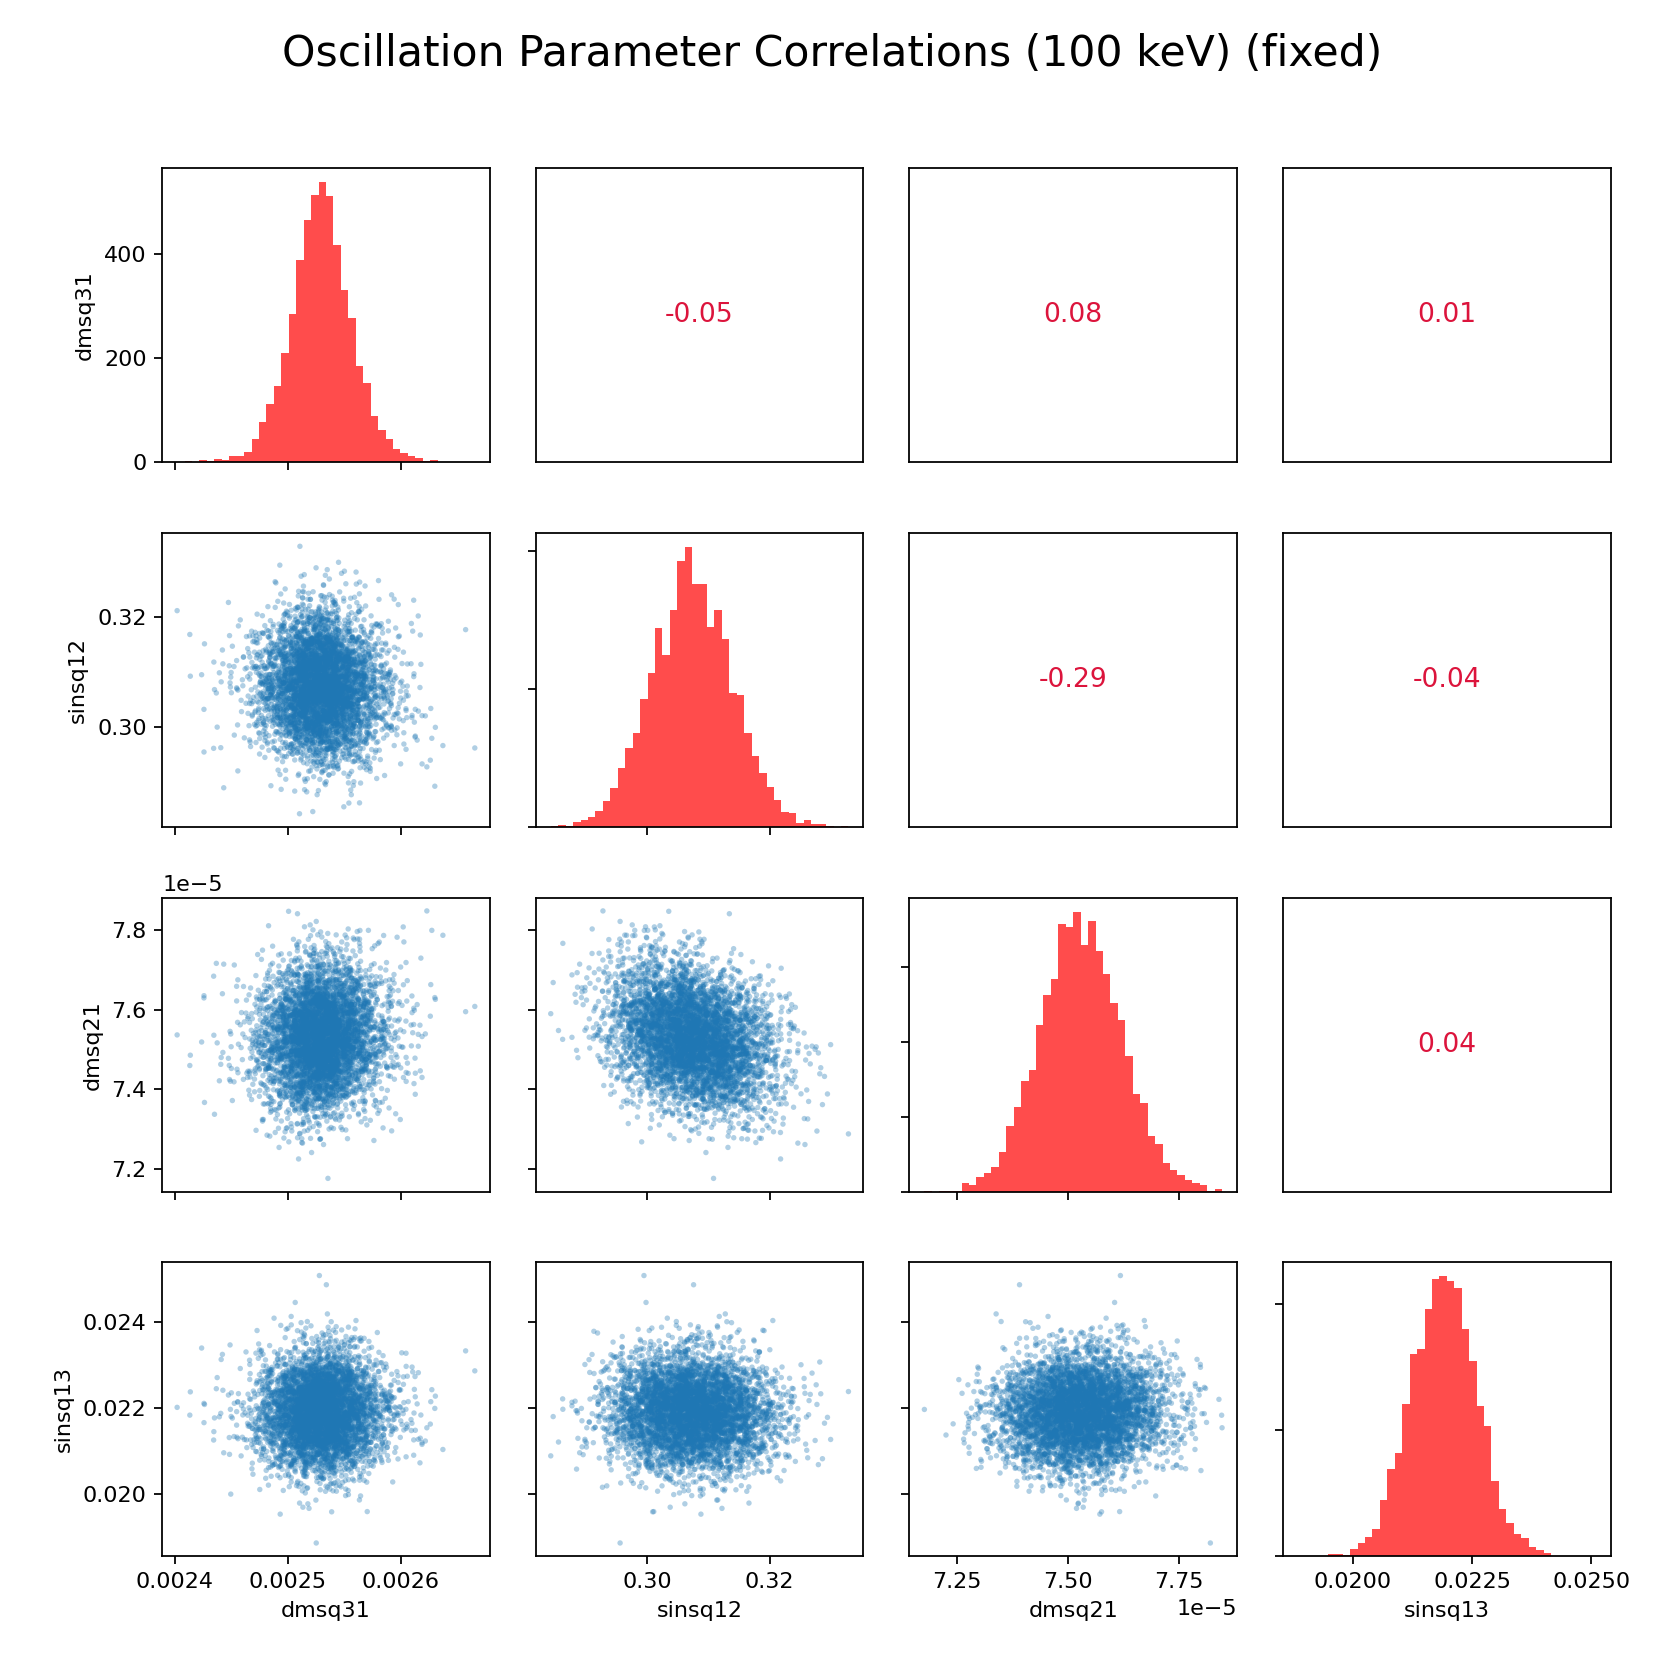
\includegraphics[width=0.75\textwidth]{Img/dmsq21_sinsq12.png}
    \bicaption{振荡参数的两两关联与边缘分布（反应堆中微子能量分段 100 keV，固定反应堆模型）。对角线为每个参数的边缘直方图；下三角为参数间散点图；上三角数值为对应的皮尔逊相关系数（图中 $\Delta m^2_{21}$ 与 $\sin^2\theta_{12}$ 的相关系数约为 $-0.29$）。这些关联说明在构造置信区间时需要考虑参数间的耦合，因此对太阳区参数采用二维 FC 构造更为合适。}{Pairwise correlations and marginal distributions of the oscillation parameters (reactor neutrino energy binning 100 keV, fixed reactor model). Diagonal panels show marginal histograms for each parameter; lower-triangular panels show pairwise scatter plots; upper-triangular entries report the corresponding Pearson correlation coefficients (the correlation between $\Delta m^2_{21}$ and $\sin^2\theta_{12}$ is about $-0.29$). These correlations motivate the use of a 2D Feldman–Cousins construction for the solar-sector parameters to properly account for their coupling when producing confidence intervals.}
    \label{fig:osc_param_corr}
  \end{figure}

图~\ref{fig:FC21} 给出在参数平面中某代表性格点处得到的经验 $\Delta\chi^2$ 分布。提取到的 68.27\% 置信水平下的临界值在统计不确定度范围内与 Wilks 期望值一致（$\chi^2(ndf = 1)$，1$\sigma$的临界值$\Delta\chi^2 \approx  2.3$）。因此，对于太阳区参量 $(\Delta m^2_{21},\sin^2\theta_{12})$，在所测试的参数区间内，Wilks 近似是充足的，可以用常规定义的卡方临界值来构造置信域。

\begin{figure}[h]
  \centering
  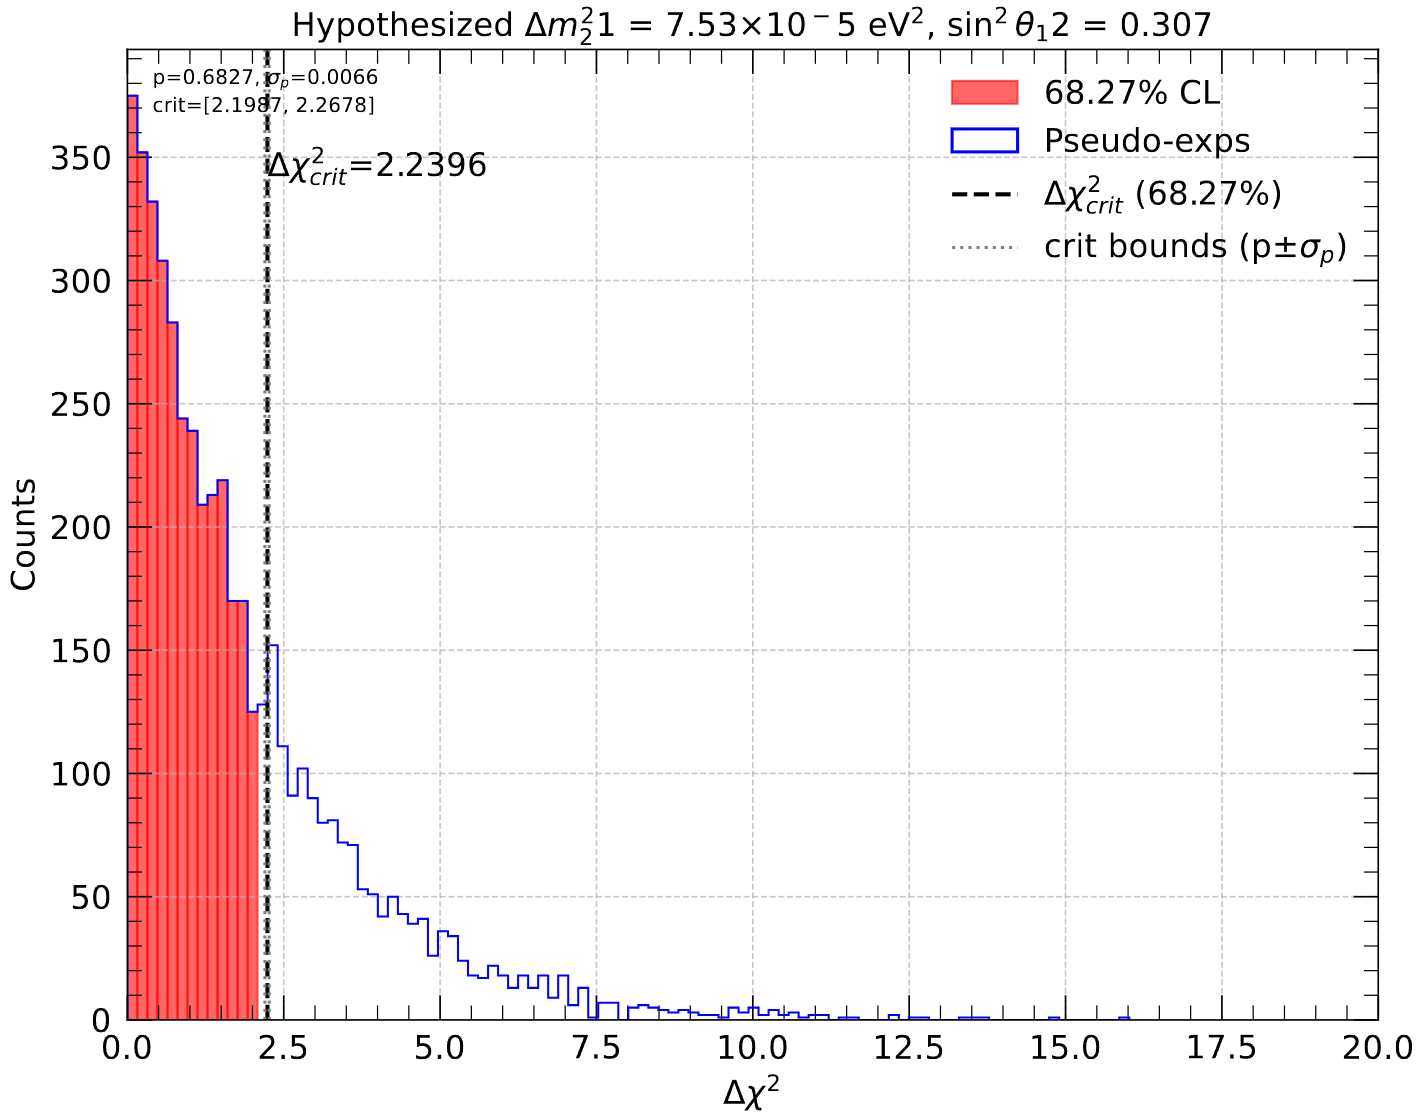
\includegraphics[width=0.7\linewidth]{Img/FC21.png}
  \bicaption[50天统计量下，二维 Feldman--Cousins 检验的经验 $\Delta\chi^2$ 分布]
  {来自二维 Feldman--Cousins 检验（在 $(\Delta m^2_{21},\,\sin^2\theta_{12})$ 参数平面某代表点处）的经验 $\Delta\chi^2$ 分布。虚线竖线指示 68.27\% 置信水平下的临界值，结果与自由度为 2 的 Wilks 期望相符。}
  {Empirical $\Delta\chi^2$ distribution from the 2D Feldman--Cousins test at a representative point in the $(\Delta m^2_{21},\,\sin^2\theta_{12})$ parameter space. The vertical dashed line indicates the critical value at 68.27\% C.L., which agrees with the Wilks expectation of a two-degrees-of-freedom $\chi^2$ distribution.}
  \label{fig:FC21}
\end{figure}

\subsection{对 $\Delta m^2_{31}$ 的一维 Feldman--Cousins}  
相比之下，$\Delta m^2_{31}$ 的似然面表现出非正则行为（附近存在非物理的低值极小与相位简并效应），这使得在纯 JUNO 配置下直接使用 Wilks 近似不再可靠。因此我们对 $\Delta m^2_{31}$ 采用一维 FC 构造。为评估反应堆谱模型依赖的影响，FC 构造分两步进行：

\begin{enumerate}  
\item \textbf{固定反应堆模型：} 设反应堆谱固定为平均 Summation Model（不做谱形扰动），在该条件下生成伪实验样本并计算经验 $\Delta\chi^2$ 分布。得到的 68.27\% 接受域临界值为
\[
 \Delta\chi^2_{\rm crit,\,fixed} = 1.5379,
\]
对应 50 天曝光下 $\Delta m^2_{31}$ 的测量精度为 $1.39\%$。该固定模型下每个 toy 的精度分布如图~\ref{fig:dmsq31_fixedaveSM} 所示。  
\item \textbf{变化反应堆模型（包含谱形扰动）：} 为了包含反应堆模型的变化，我们通过对每个 20 keV 段进行扰动（构造出一族带有精细结构的替代谱），抽样生成一组被扰动的反应堆谱（采样模型集合，$N_{\rm toys}=5000$），并在这些扰动模型上重复 FC 构造。此时经验临界值变为
\[
 \Delta\chi^2_{\rm crit,\,sampled} = 1.5724,
\]
对应的 $\Delta m^2_{31}$ 精度为 $1.40\%$（50 天曝光）。采样（高斯扰动）模型下的每个 toy 精度分布见图~\ref{fig:dmsq31_gaussian}。  
\end{enumerate}

\begin{figure}[htbp]
  \centering
  \begin{subfigure}[t]{0.47\textwidth}
    \centering
    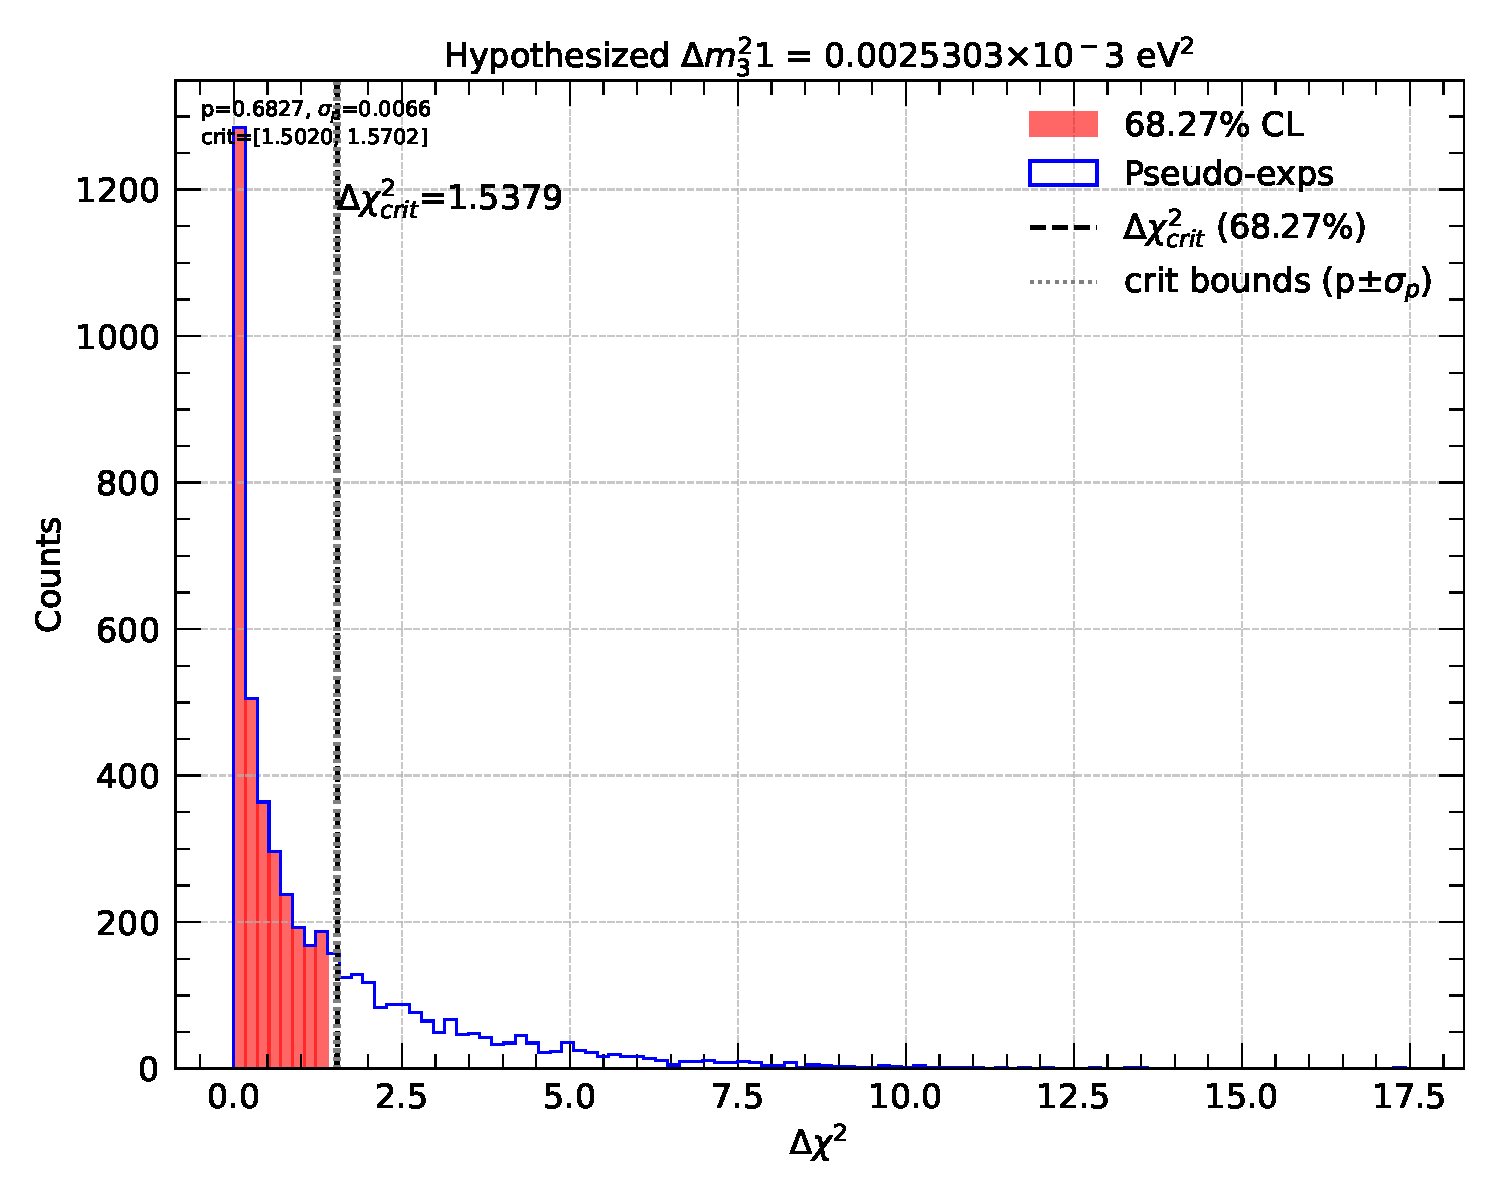
\includegraphics[width=\linewidth]{Img/segment_300_rec_100_0_0025303_dmsq31_constraint_dchi2.pdf}
    \caption{固定反应堆模型}
    \label{fig:fc_dchi2_fixed}
  \end{subfigure}
  \hfill
  \begin{subfigure}[t]{0.47\textwidth}
    \centering
    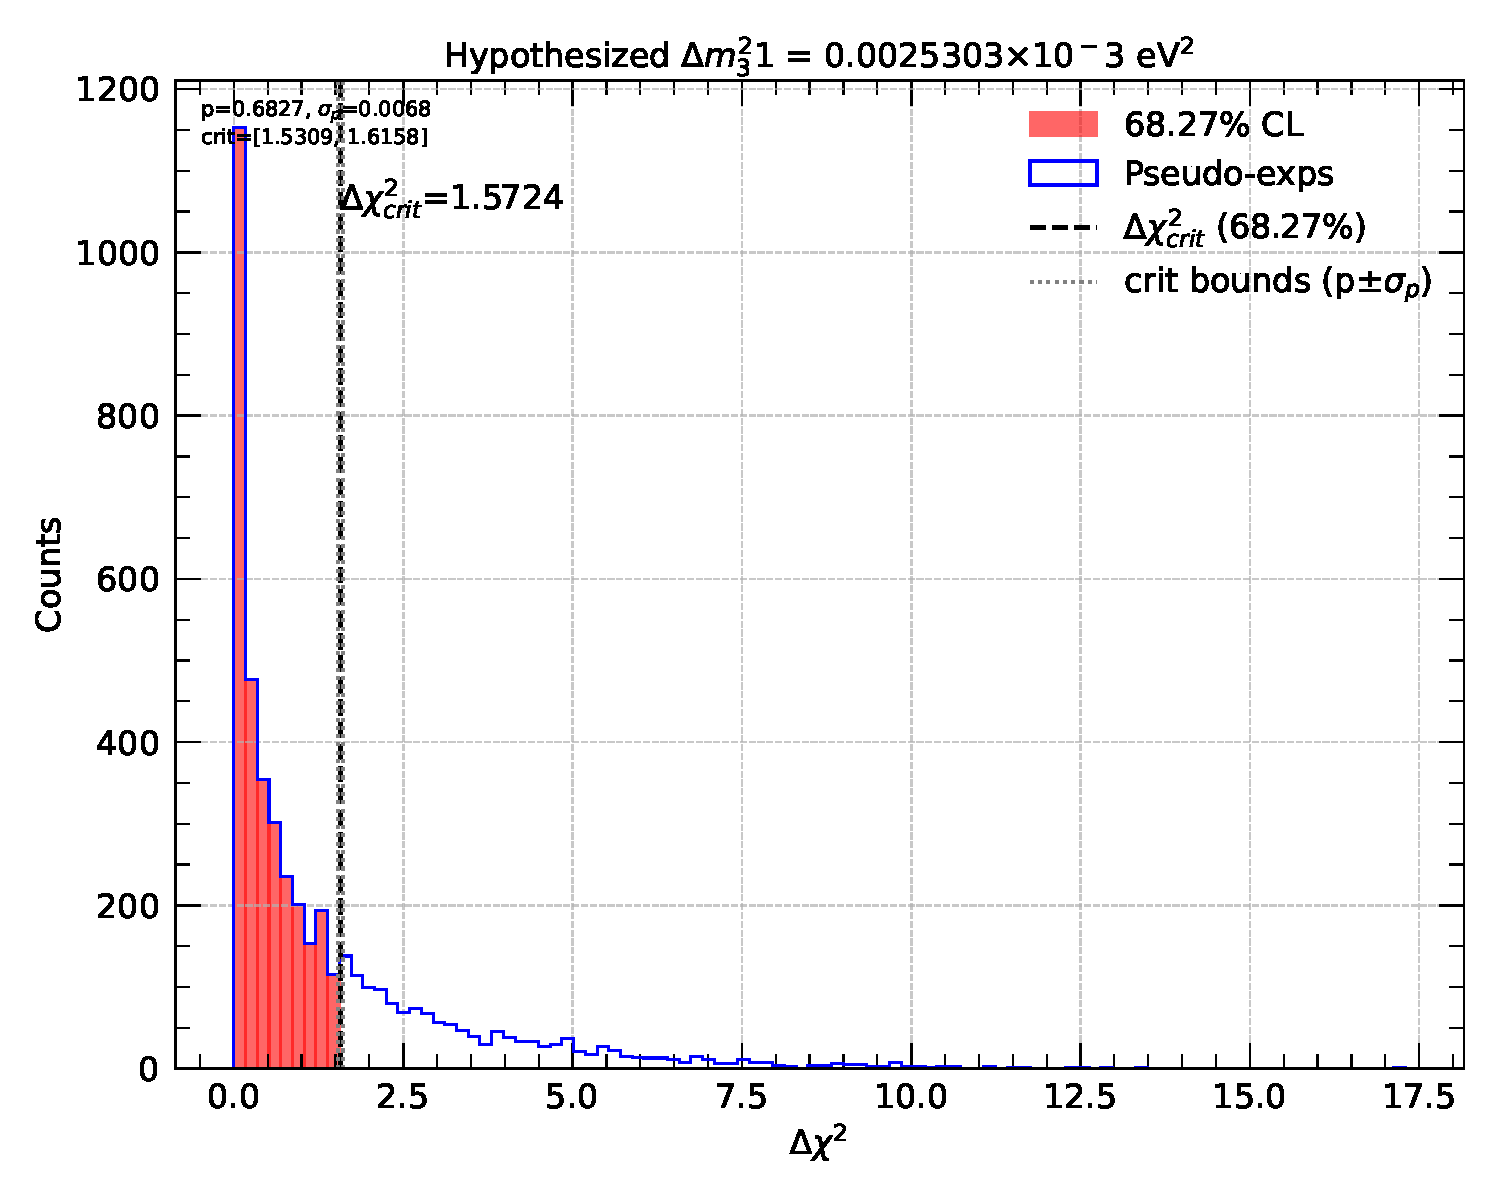
\includegraphics[width=\linewidth]{Img/segment_300_rec_100_0_0025303_dmsq31_constraint_dchi2_vary.pdf}
    \caption{变化反应堆模型}
    \label{fig:fc_dchi2_sampled}
  \end{subfigure}

  \bicaption[四种统计量下的 $\Delta m^2_{31}$ 侧向轮廓化曲线]{基于 Feldman–Cousins 构造得到的经验检验统计量 $\Delta\chi^2$ 分布（50 天统计量）。左图：固定反应堆模型下的结果；红色柱状表示被接受到 68.27\% 接受域内的伪实验（填充），蓝色轮廓为所有伪实验的分布（pseudo-exps）；虚线表示对应于 68.27\% 的经验临界值 $\Delta\chi^2_{\rm crit}=1.5379$。右面板：在扰动（sampled）反应堆模型（包含谱形细结构扰动）下的结果；对应经验临界值为 $\Delta\chi^2_{\rm crit}=1.5724$。两幅图均使用相同的横轴与归一化方式，展示了模型不确定性对经验临界值的微小影响。}
  {Empirical distributions of the test statistic $\Delta\chi^2$ obtained with the Feldman–Cousins construction (50-day exposure). Left panel: fixed reactor-model case; the red filled histogram shows the toys accepted within the 68.27\% acceptance region, while the blue outline shows the full pseudo-experiment distribution; the vertical dashed line marks the empirical critical value $\Delta\chi^2_{\rm crit}=1.5379$ (68.27\%). Right panel: sampled/perturbed reactor-model ensemble (including fine-structure perturbations); the empirical critical value in this case is $\Delta\chi^2_{\rm crit}=1.5724$. Both panels use identical axis scaling and normalization and illustrate the (small) effect of reactor-model variation on the FC-derived critical value.}
  \label{fig:dmsq31_FC_histograms}
  \label{fig:fc_dchi2_fixed_vs_sampled}
\end{figure}

当采用采样的反应堆模型集合时，经验临界值较固定模型略有上升，但差别较小；且通过增加 FC 中的伪实验数量可以进一步降低经验临界值的统计不确定性。

由上述研究可得出以下结论：  
\begin{itemize}  
\item 反应堆模型变化对 $\Delta m^2_{31}$ 的附加系统贡献很小：在 50 天情形下估计该项对 $\Delta m^2_{31}$ 精度的影响小于 $0.3\%$。  
\item 对三项参数（$\Delta m^2_{21}$, $\sin^2\theta_{12}$, $\Delta m^2_{31}$）而言，在 50 天曝光下由现实可行的反应堆模型变化引入的系统不确定度均小于统计不确定度；即在该曝光下模型相关系统误差可视为次要。  
\item 在所采用的假设下，基于 FC 的 $\Delta m^2_{31}$ 精度约为 $1.4\%$（50 天），略差于全局拟合给出的约 $1.1\%$ 的精度，但在仅用 JUNO 数据并考虑反应堆模型不确定性的内部一致性下该结果是合理的。  
\end{itemize}

\begin{figure}[!htbp]  
\centering  
\begin{subfigure}[t]{0.45\textwidth}  
\centering  
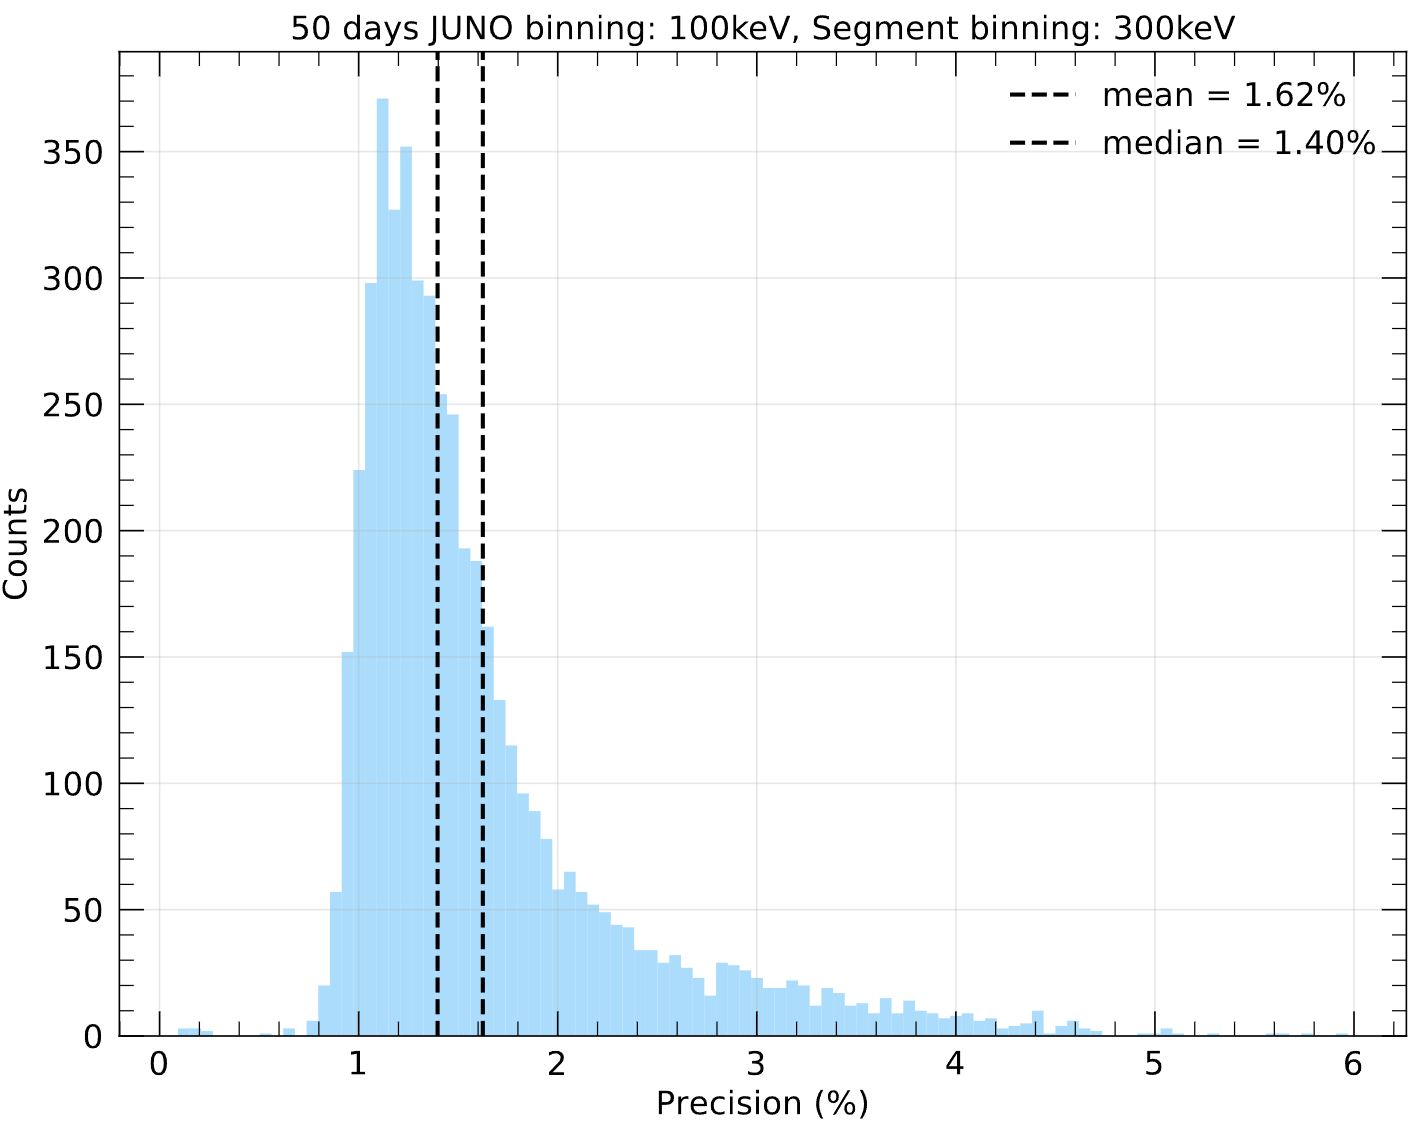
\includegraphics[width=\linewidth]{Img/dmsq31_gaussian.png}  
\bicaption{变化反应堆模型集合下的每个 toy 精度分布（$N_{\rm toys}=5000$）。}{Per-toy precision distribution for the sampled  reactor-model ensemble ($N_{\rm toys}=5000$).}  
\label{fig:dmsq31_gaussian}  
\end{subfigure}%  
\hfill  
\begin{subfigure}[t]{0.45\textwidth}  
\centering  
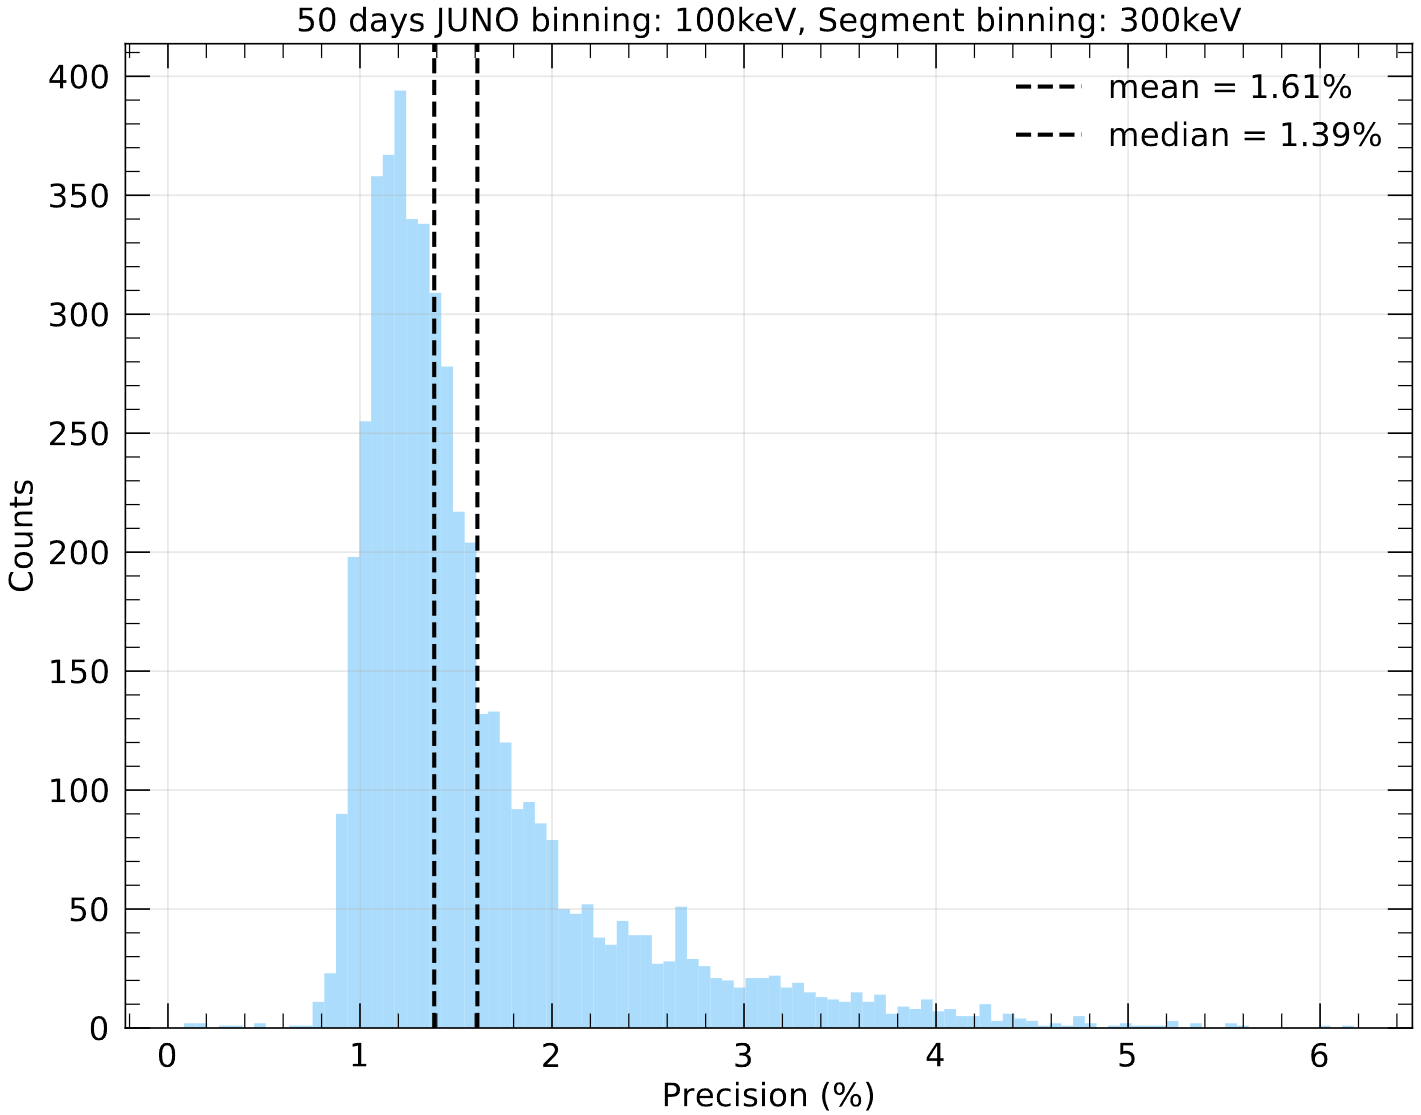
\includegraphics[width=\linewidth]{Img/dmsq31_fixedaveSM.png}  
\bicaption{固定平均 Summation Model（无谱形扰动）情形下的每个 toy 精度分布（$N_{\rm toys}=5000$）。}{Per-toy precision distribution for the fixed average Summation Model ($N_{\rm toys}=5000$) (no shape perturbation).}  
\label{fig:dmsq31_fixedaveSM}  
\end{subfigure}  
\caption{用于评估 $\Delta m^2_{31}$ 精度与模型敏感性的 per-toy 精度分布比较（左：采样模型；右：固定模型）。}  
\label{fig:dmsq31_FC}  
\end{figure}

\subsection{Feldman--Cousins 临界值对 \texorpdfstring{$\Delta m^2_{31}$}{Delta m2\_31} 扫描区间的依赖性}
\begin{figure}[h]
  \begin{subfigure}[t]{0.47\textwidth}
    \centering
    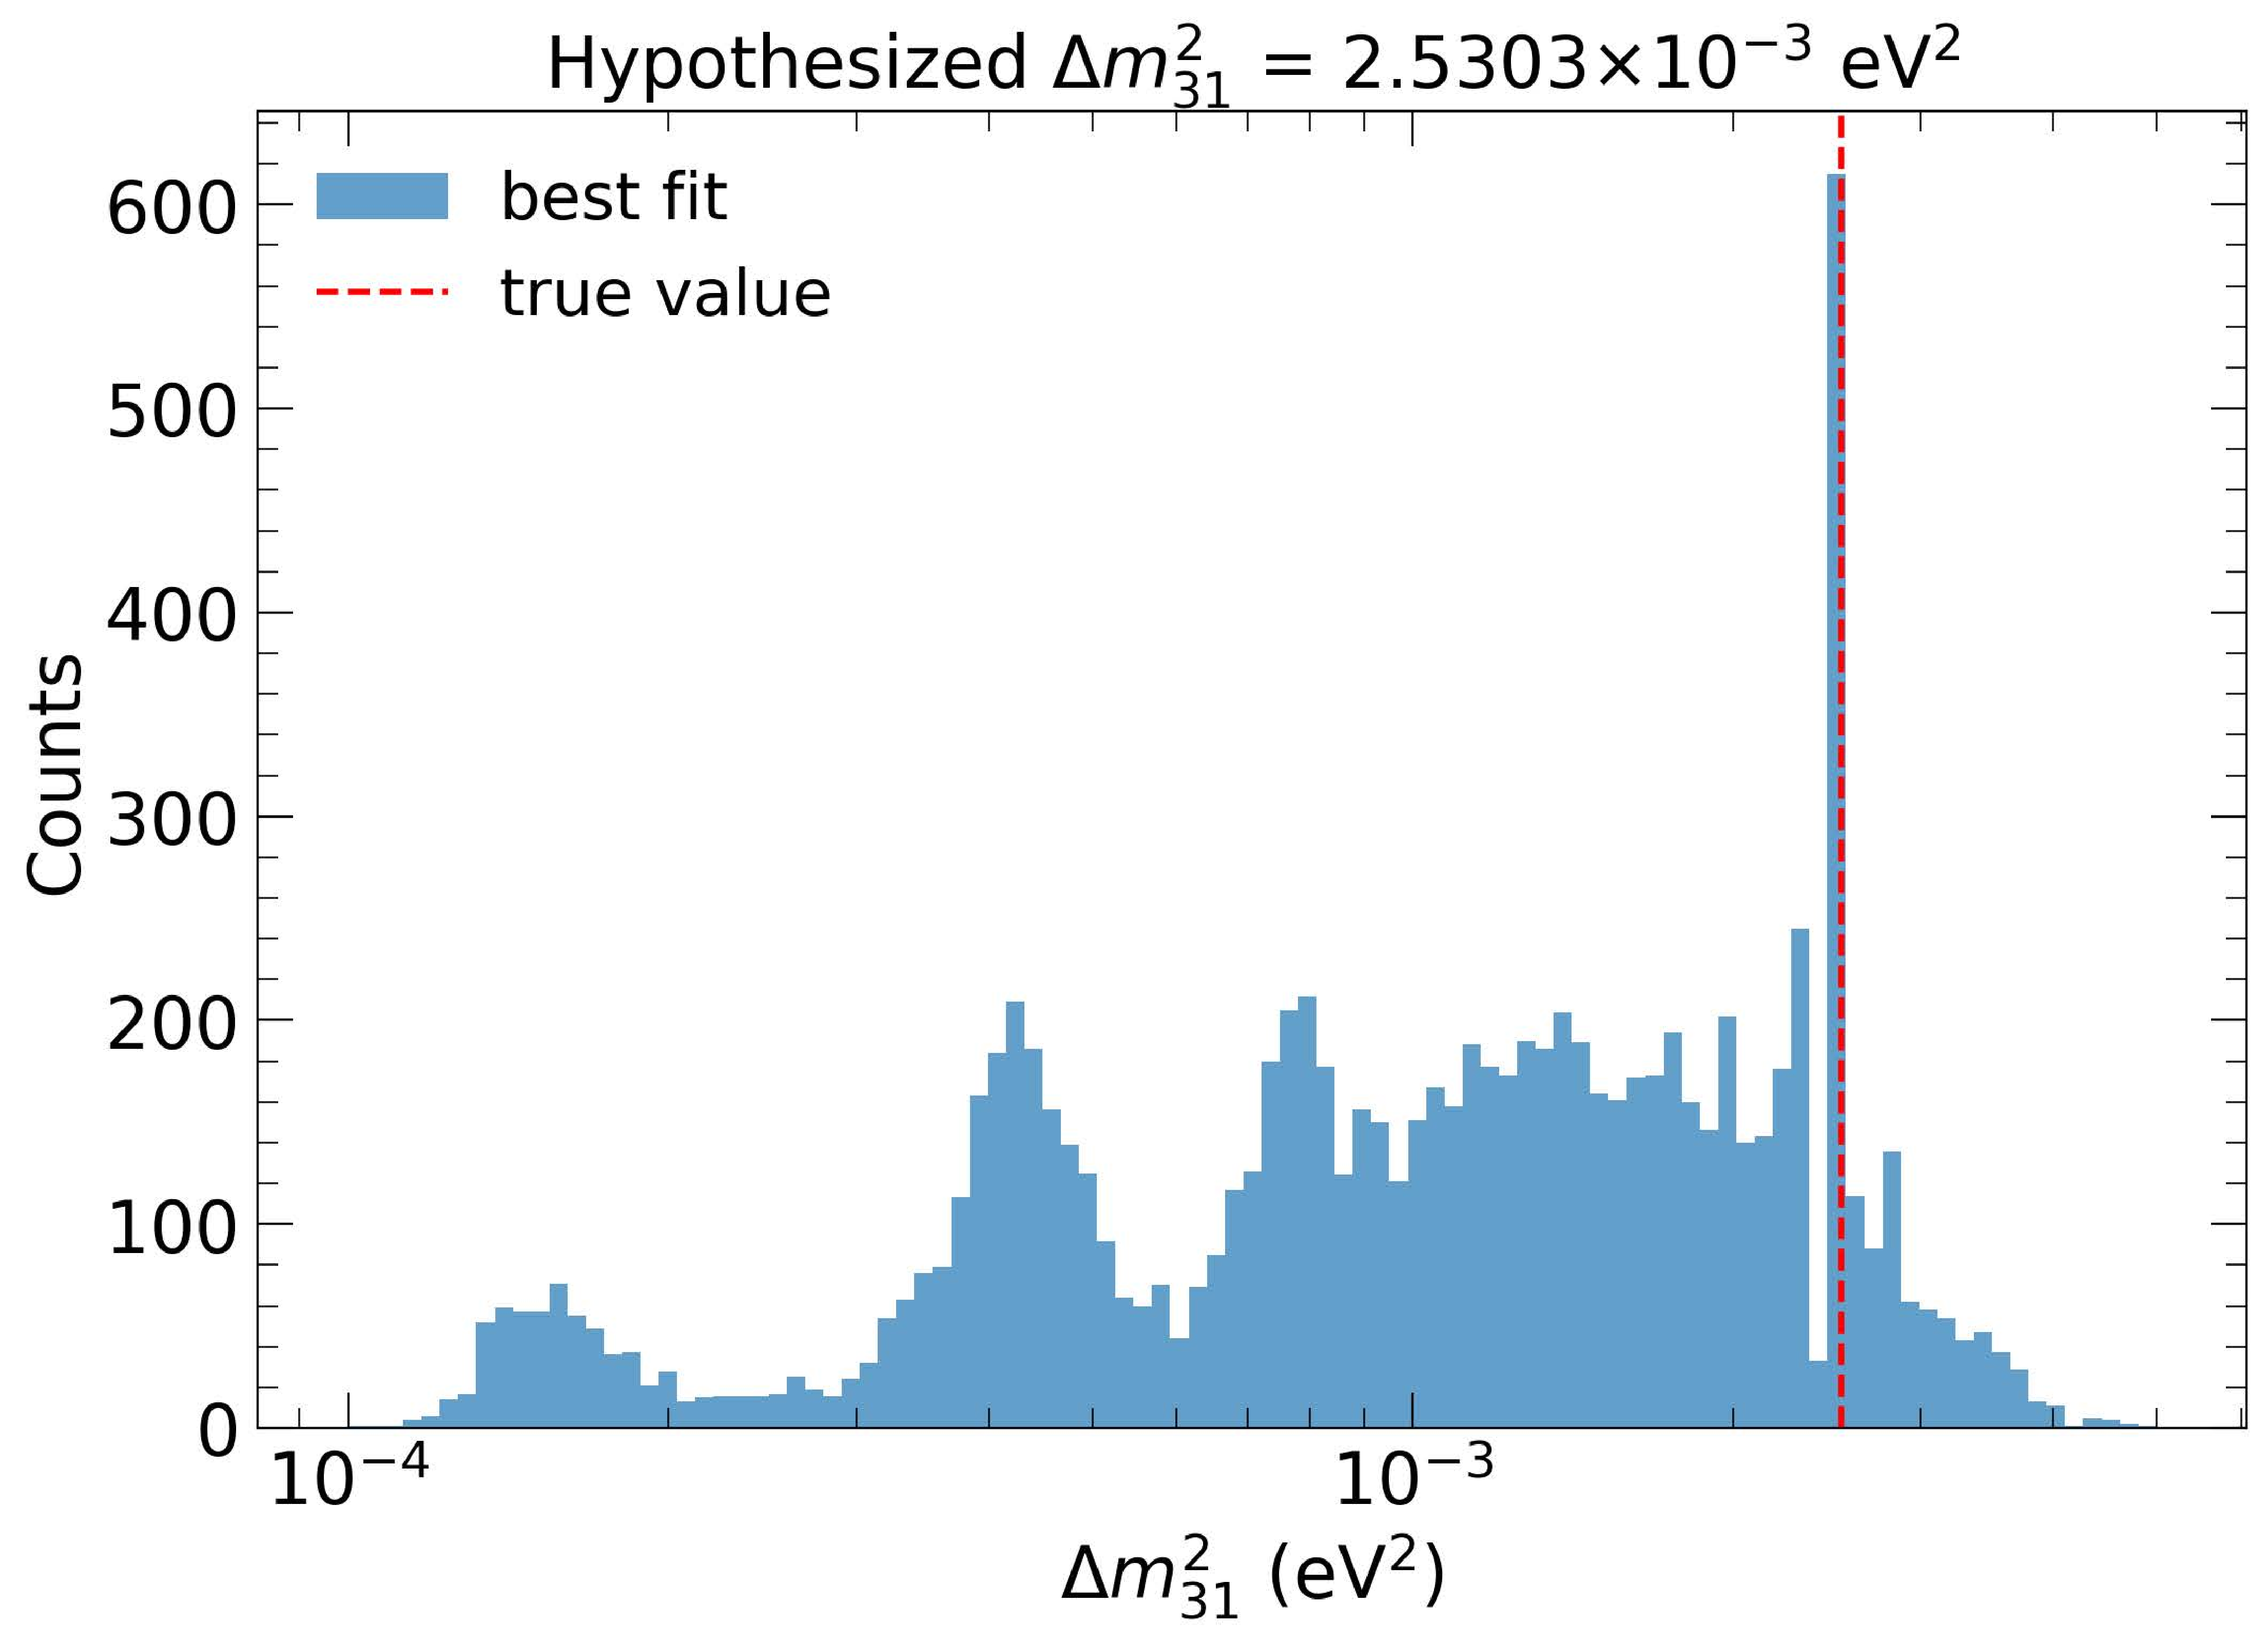
\includegraphics[width=\linewidth]{Img/Jingqin_dmsq31_bestfit_distribution.pdf}
    \caption{Distribution of Best-Fit $\Delta m^2_{31}$ from Toy MC}
    \label{fig:dmsq31_best_fit_distribution}
  \end{subfigure}
  \hfill
  \begin{subfigure}[t]{0.47\textwidth}
    \centering
    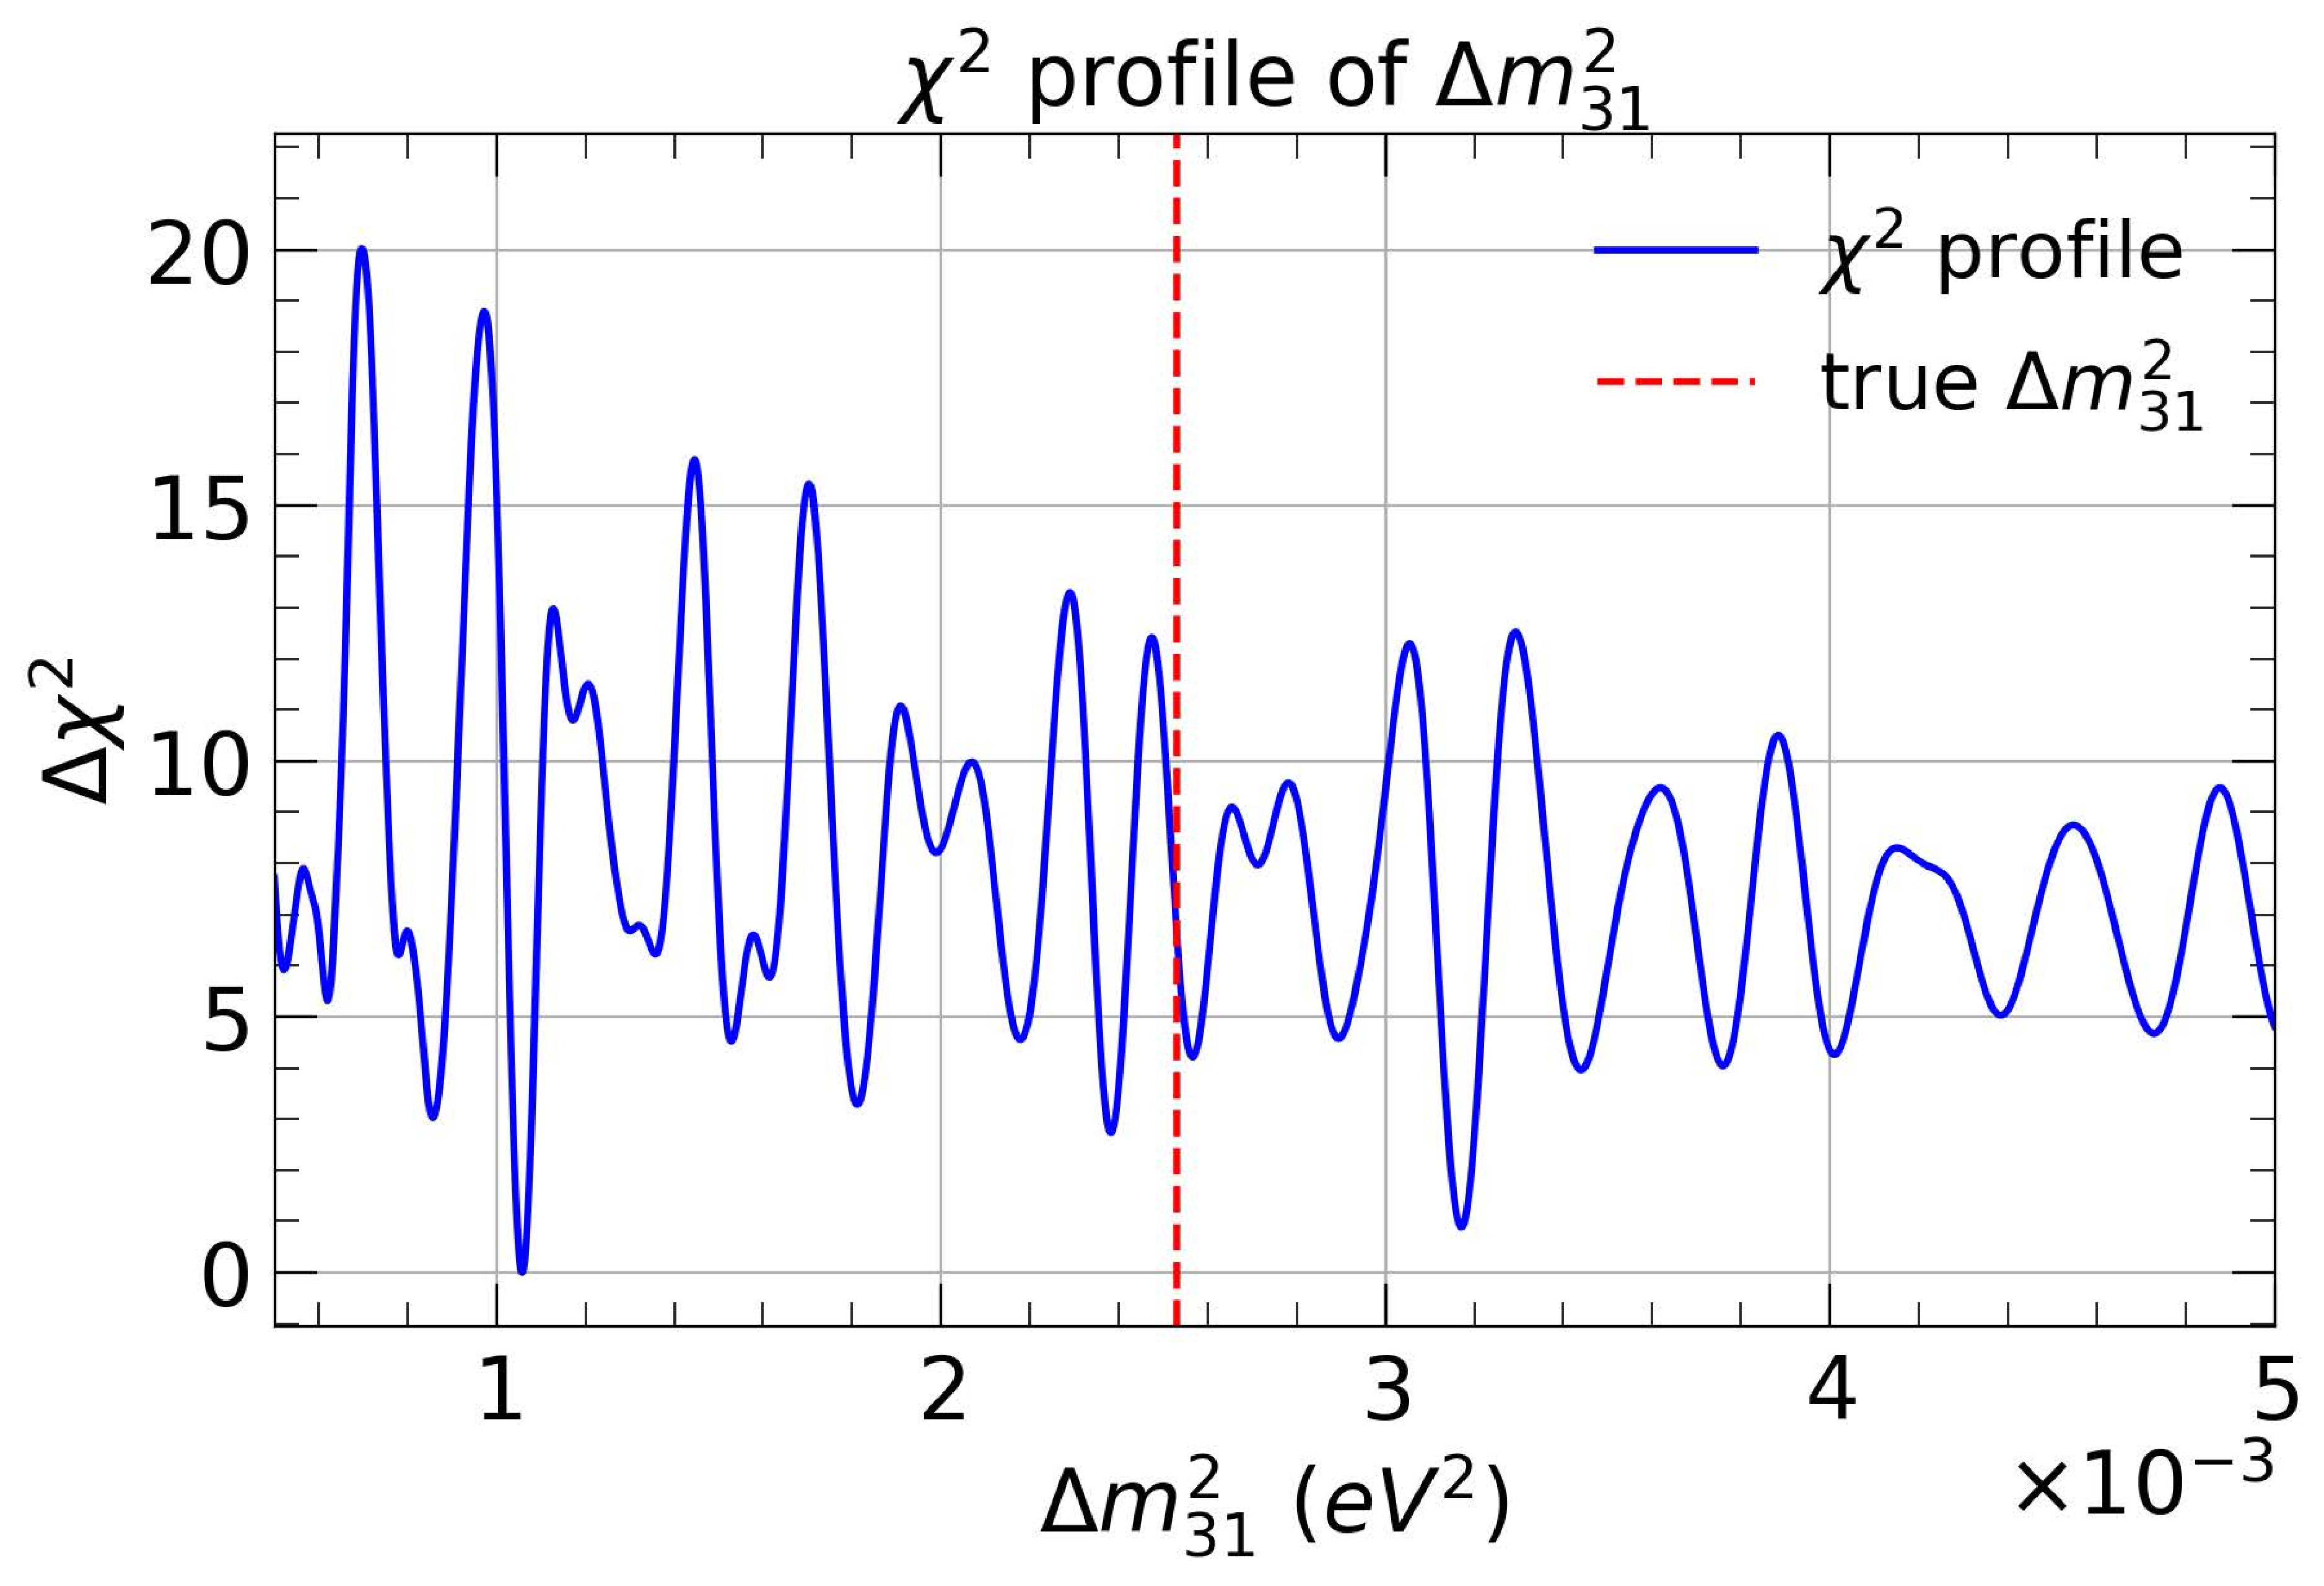
\includegraphics[width=\linewidth]{Img/Jingqin_toy_data.pdf}
    \caption{$\chi^2$ Profile of $\Delta m^2_{31}$ from a Single Toy Dataset}
    \label{fig:toy_data_profile}
  \end{subfigure}
  \bicaption{(a) 由一组伪实验（Toy MC）得到的 $\Delta m^2_{31}$ 最优拟合值分布直方图（30 天曝光）。横轴为最优拟合的 $\Delta m^2_{31}$（单位 eV$^2$，对数尺度），红色虚线标示注入的真值。(b) 来自单一伪实验的数据的 $\Delta\chi^2(\Delta m^2_{31})$ 轮廓。横轴为扫描的 $\Delta m^2_{31}$ 值（eV$^2$），纵轴为相对其最小值的 $\Delta\chi^2$。蓝色曲线呈现多个局域极小值并明显偏离二次抛物形；红色虚线为真值。}{(a) Histogram of best-fit $\Delta m^2_{31}$ values obtained from an ensemble of toy Monte Carlo experiments under 30 days exposure. The horizontal axis shows the best-fit $\Delta m^2_{31}$ (eV$^2$; log scale), and the vertical axis gives the number of best-fit values falling in each bin. The red dashed line marks the true (injected) value. (b) $\Delta\chi^2(\Delta m^2_{31})$ profile from a single toy dataset whose global minimum lies far from the true value. The horizontal axis is the scanned $\Delta m^2_{31}$ (eV$^2$); the vertical axis is $\Delta\chi^2$ relative to its minimum. The blue curve exhibits multiple local minima and markedly non-quadratic behavior; the red dashed line denotes the true value.}
  \label{fig:dmsq31_best_fit}
\end{figure}
在低统计量情况下，图~\ref{fig:dmsq31_best_fit} 清楚地表明：来自伪实验的 $\Delta m^2_{31}$ 最优拟合值可以显著偏离输入的真值；且对某一代表性伪实验绘制的 $\chi^2$ 轮廓（右图）表现出高度非二次的行为并包含大量局域极小值。
\begin{figure}[h]
  \begin{subfigure}[t]{0.47\textwidth}
    \centering
    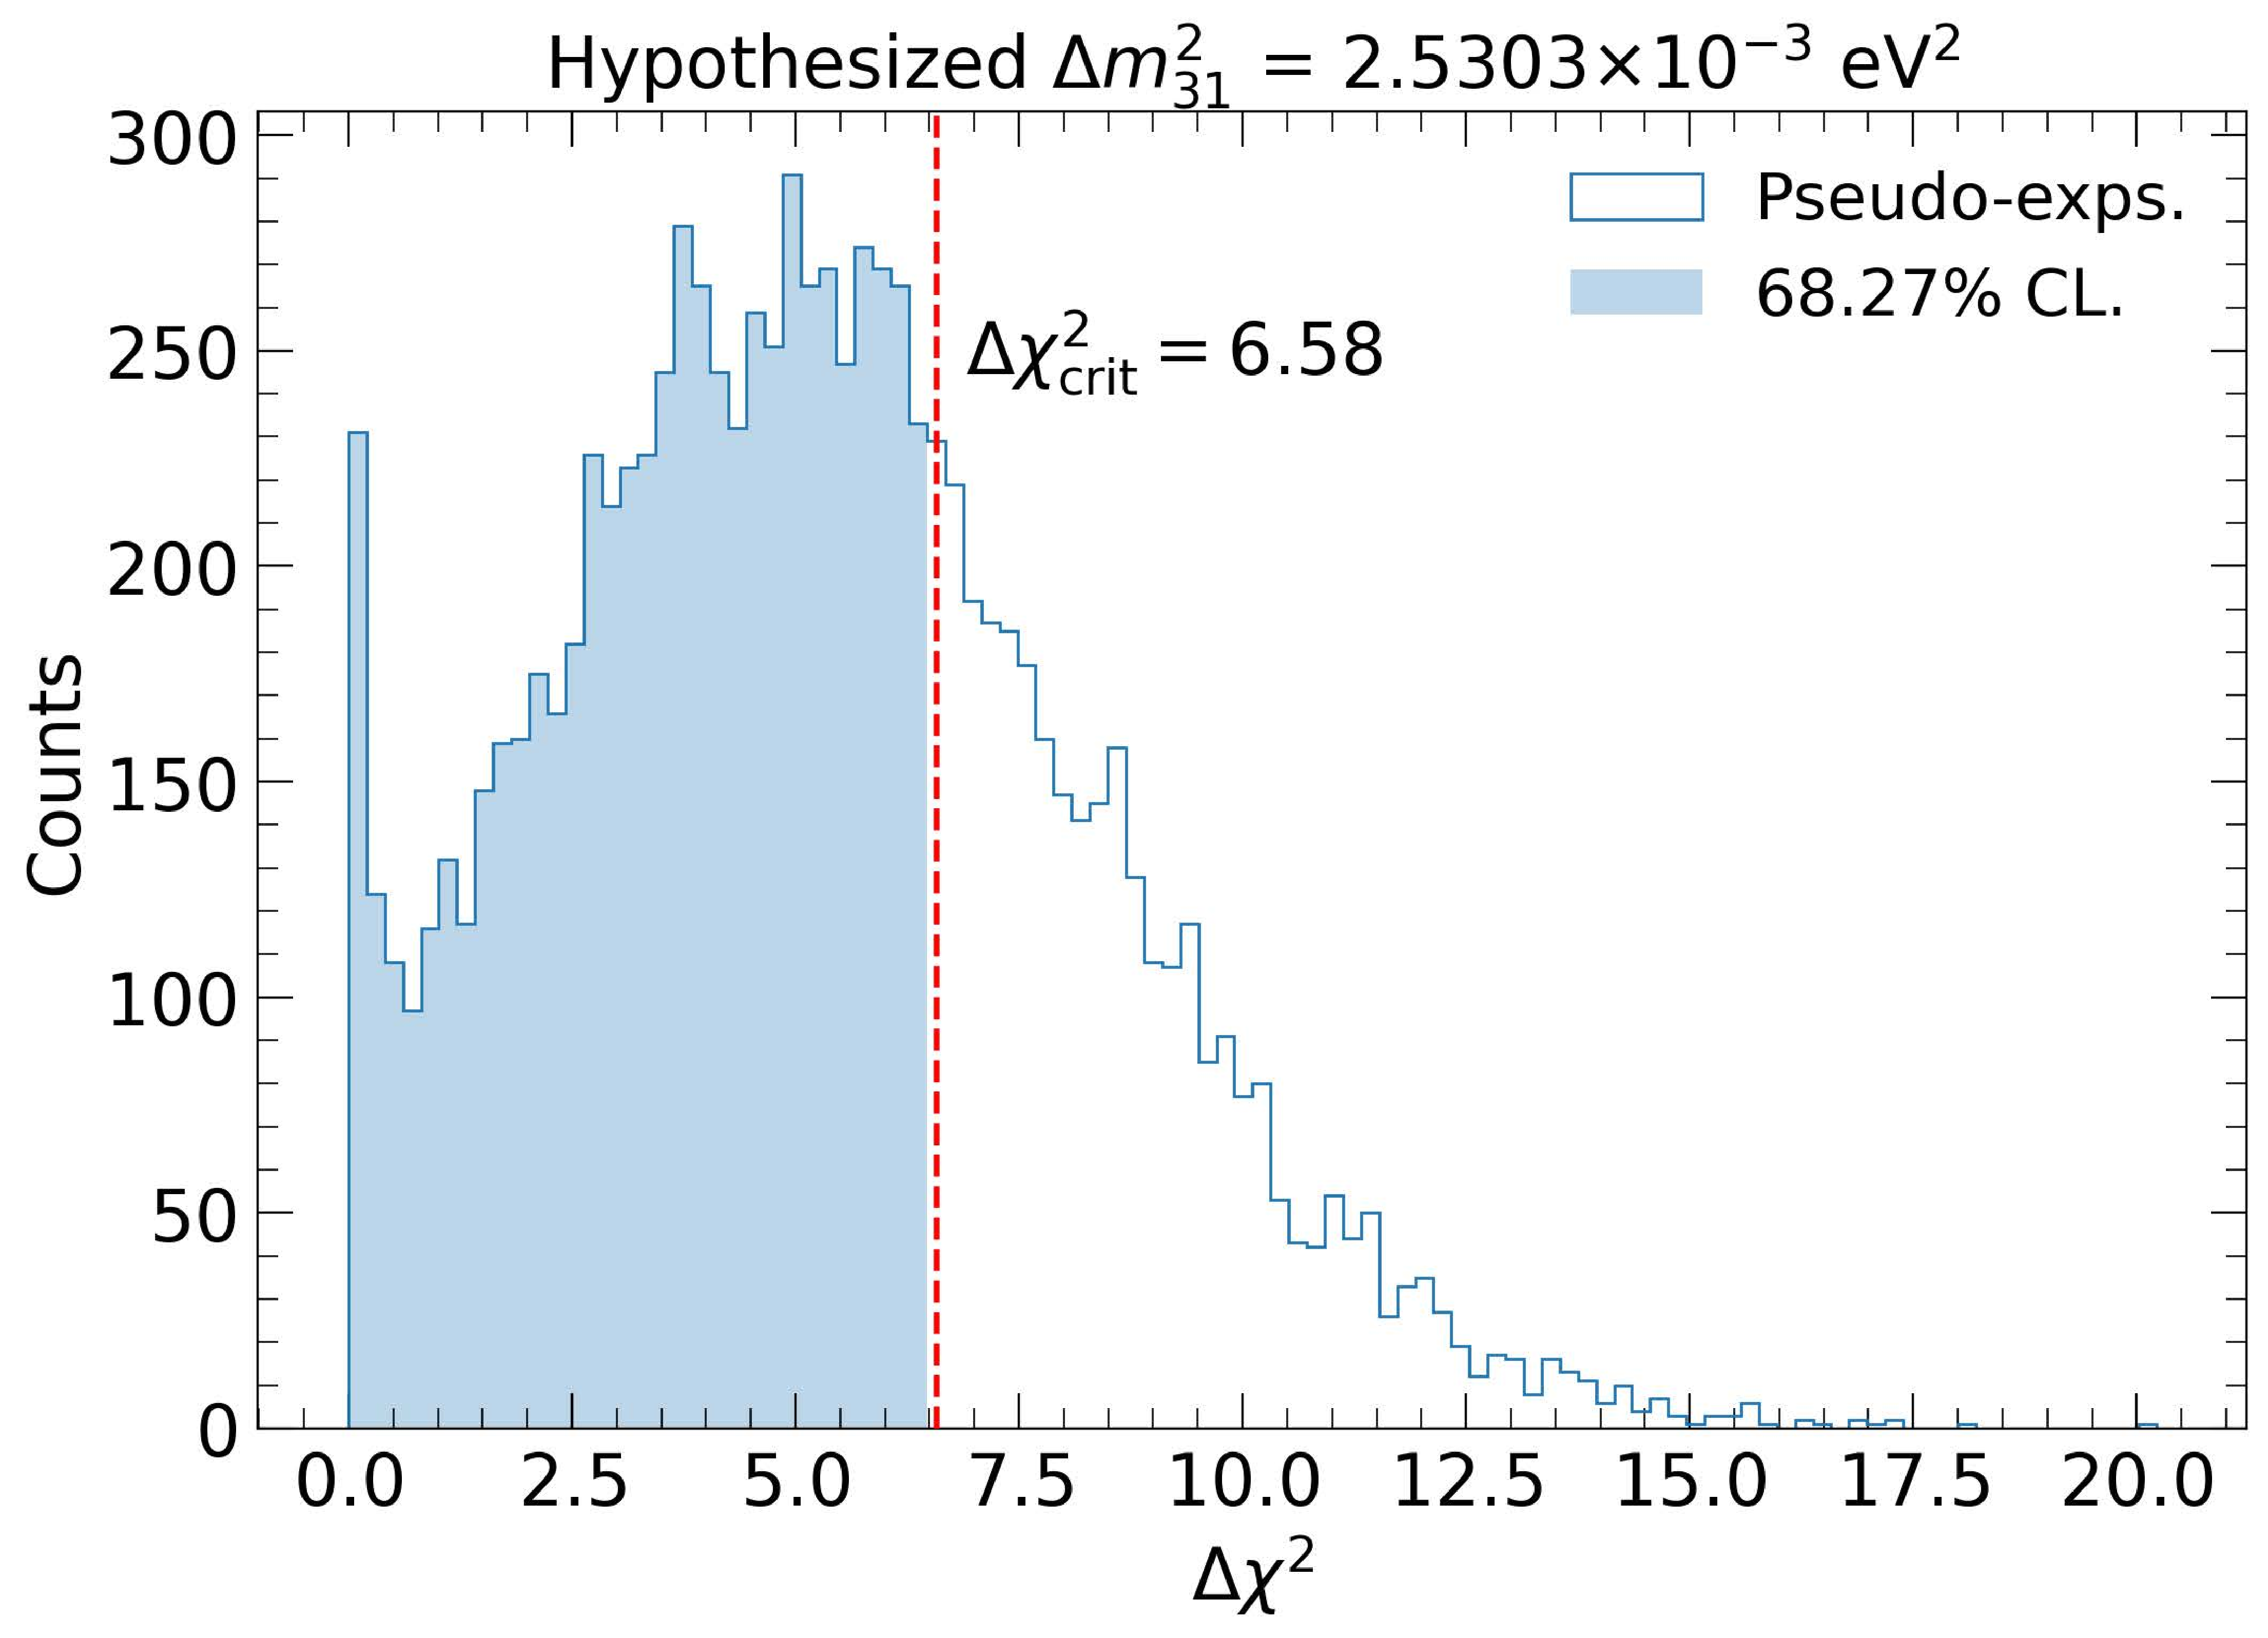
\includegraphics[width=\linewidth]{Img/Jingqin_big_range_dchi2.pdf}
    \caption{$\Delta m^2_{31} \in [1.0 \times 10^{-4}, 5.0 \times 10^{-3}]$ eV$^2$}
    \label{fig:big_range_dchi2_distribuiton}
  \end{subfigure}
  \hfill
  \begin{subfigure}[t]{0.47\textwidth}
    \centering
    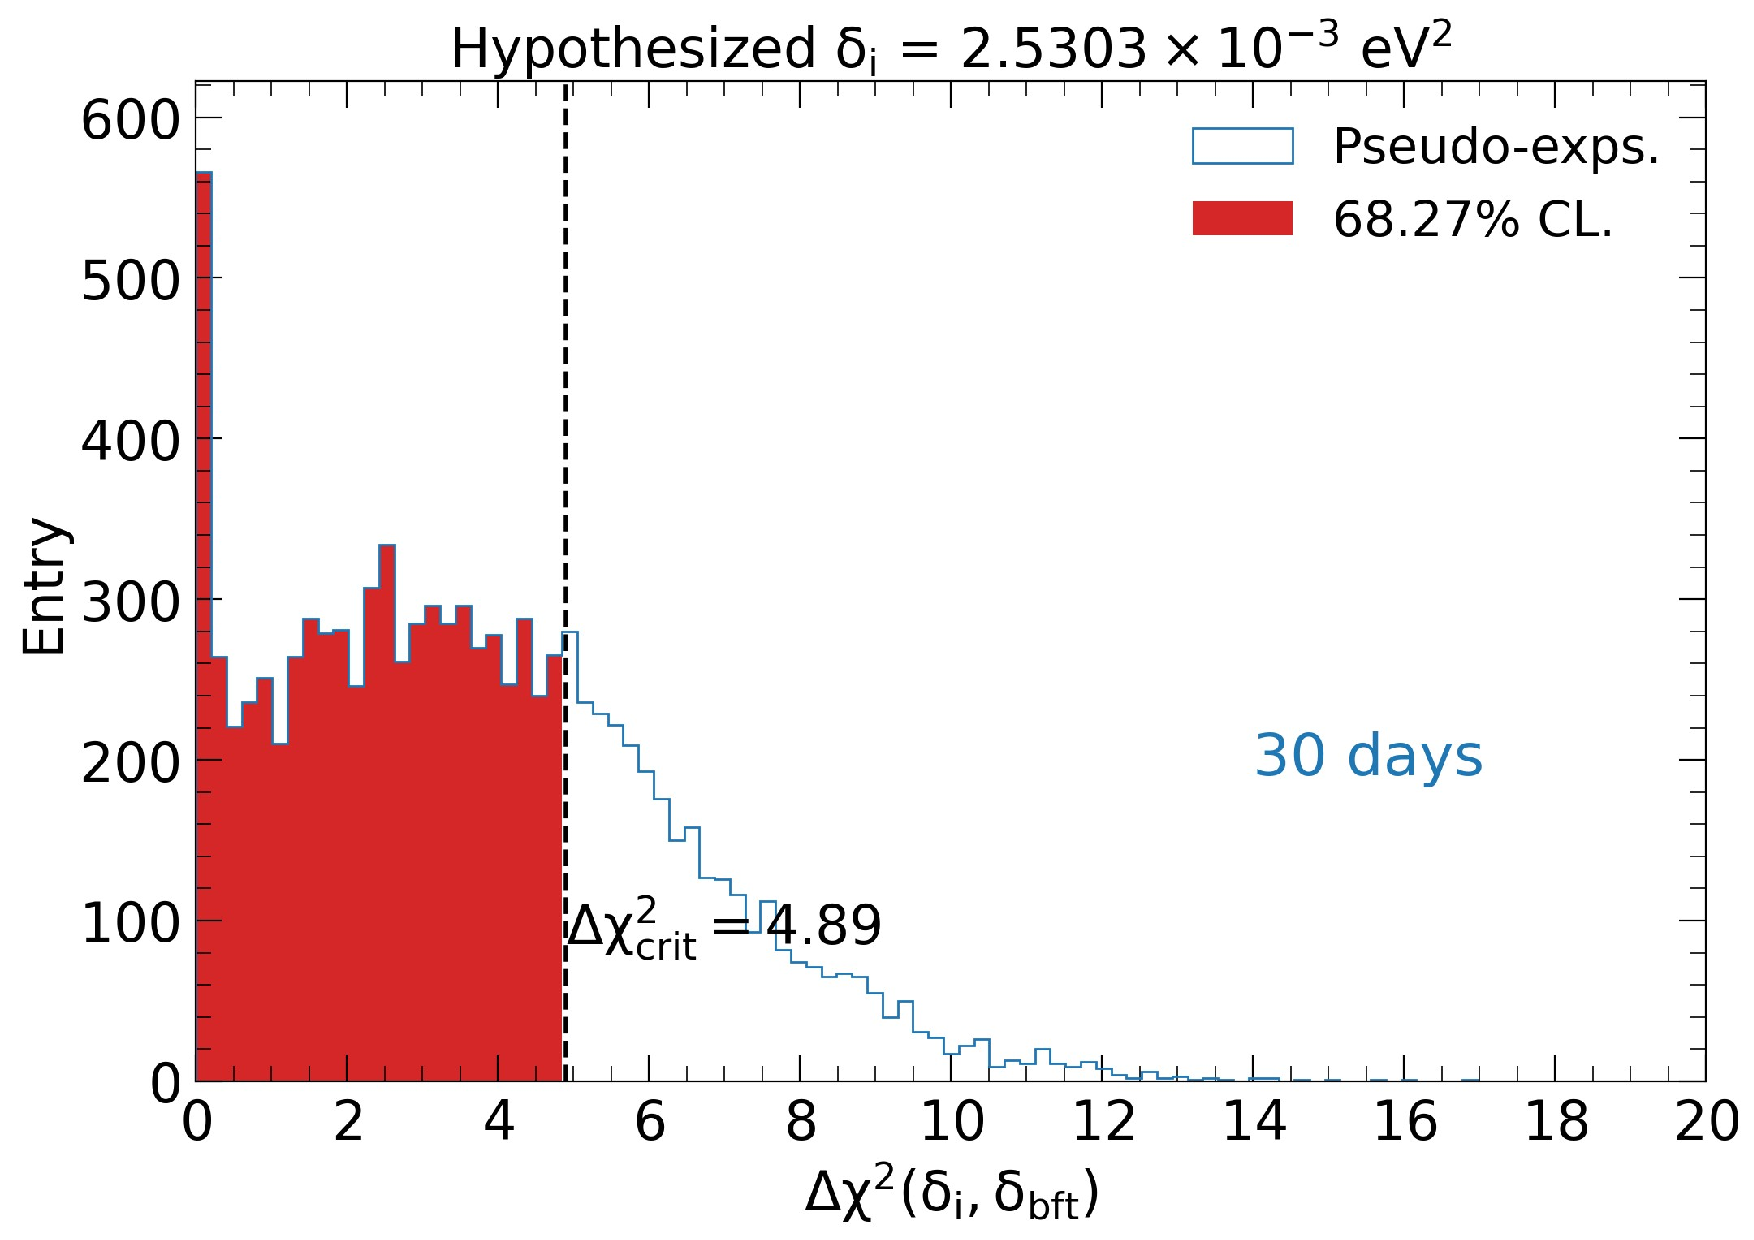
\includegraphics[width=\linewidth]{Img/Jingqin_small_range_dchi2.pdf}
    \caption{$\Delta m^2_{31} \in [1.5 \times 10^{-3}, 3.5 \times 10^{-3}]$ eV$^2$}
    \label{fig:small_range_dchi2_distribution}
  \end{subfigure}
  \bicaption{基于伪实验得到的 Feldman–Cousins 检验统计量 $\Delta\chi^2$ 的经验分布（注入真值 $\Delta m^2_{31}=2.5303\times10^{-3}\,\mathrm{eV}^2$）。(a) 使用较大扫描区间 $[1\times10^{-4},\,5\times10^{-3}]\,\mathrm{eV}^2$，此时得到的经验临界值（68.27\%）为 $\Delta\chi^2_{\rm crit}=6.58$；(b) 使用较窄扫描区间 $[1.5\times10^{-3},\,3.5\times10^{-3}]\,\mathrm{eV}^2$，此时的经验临界值为 $\Delta\chi^2_{\rm crit}=4.89$。横轴为 $\Delta\chi^2$ 值，纵轴为产生该 $\Delta\chi^2$ 的伪实验计数。阴影蓝区为对应 68.27\% 的中心分位区间（FC 的 1σ 接受域）。虚线表示传统 Wilks 假设下的 $\Delta\chi^2=1$。}{Distribution of the Feldman–Cousins test statistic $\Delta\chi^2$ obtained from pseudo-experiments generated under the hypothesis true value $\Delta m^2_{31} = 2.5303\times10^{-3} \,\mathrm{eV}^2$ (yielding $\Delta\chi^2_{\rm crit}=6.58$). (a) Large scan range: the $\Delta m^2_{31}$ scan was performed over $[1\times10^{-4},\,5\times10^{-3}]\,\mathrm{eV}^2$. (b) Narrow scan range: the $\Delta m^2_{31}$ scan was performed over $[1.5\times10^{-3},\,3.5\times10^{-3}]\,\mathrm{eV}^2$ (yielding $\Delta\chi^2_{\rm crit}=4.89$). The horizontal axis shows the $\Delta\chi^2$ values, and the vertical axis indicates the number of pseudo-experiments yielding a given $\Delta\chi^2$ value. The histogram represents the full distribution from all pseudo-experiments. The shaded blue area marks the central 68.27\% quantile range, corresponding to the one-standard-deviation ($1\sigma$) confidence level in the Feldman–Cousins construction. The vertical dashed line indicates the conventional $\Delta\chi^2 = 1$ threshold assumed under Wilks’ theorem.}
  \label{fig:dmsq31_dchi2_distribution}
\end{figure}

图~\ref{fig:dmsq31_dchi2_distribution} 显示：在低统计量情形下，传统的 Wilks 阈值 $\Delta\chi^2=1$ 明显低估了真实的不确定度；通过伪实验得到的 FC 经验临界值往往要大得多。此外，FC 临界值对所扫掠的 $\Delta m^2_{31}$ 区间长度敏感——若扫描区间过窄，可能会遗漏替代的全局极小值，从而使某些伪实验的 $\Delta\chi^2$ 统计量被低估，导致覆盖率不足（undercoverage）。由此可见，在用 Feldman–Cousins（FC）方法构造 $\Delta\chi^2$ 分布时，需要对初始拟合起点采用宽广的扫描区间并使用多个起始值，以保证找到全局最优解，避免拟合陷入局域极小值，从而确保 FC 构造的覆盖率正确。

\section{本章小节}
\label{sec:FC_summary}
本章首先聚焦于在 JUNO 早期低统计量情形下置信区间构造的可靠性问题。我们指出 Asimov 灵敏度不能再现真实数据中由统计涨落引起的非平稳性——例如 $\Delta m_{31}^2$ 轮廓上常见的多个局域极小值（“bad minima”）和由此产生的多段不连续置信区间。针对这一现实情况，章中系统地回顾了 Wilks 定理的适用前提并阐明其在本问题中的局限性，进而引入 Feldman–Cousins（FC）方法：通过在每一待测参数点生成大量包含统计与系统误差涨落的伪实验、对每个伪实验重复完整拟合流程，以经验分布的方式求取 $\Delta\chi^2$ 的临界值，从而在不依赖渐近近似的前提下保证频率学覆盖。

基于上述思路，我们开展了大规模的覆盖性研究。对太阳区参数（$\Delta m^2_{21}$、$\sin^2\theta_{12}$）采用二维 FC 构造，结果表明在所测试的参数区域与统计量条件下经验 $\Delta\chi^2$ 与自由度为 2 的卡方分布相符，因此可安全使用常规定阈值（1σ 对应 $\Delta\chi^2\approx 2.3$）构造置信域。相对地，对 $\Delta m^2_{31}$ 的一维 FC 构造得到的结论则不同：在固定反应堆模型下 50 天情形的经验 68.27\% 临界值约为 $\Delta\chi^2_{\rm crit}\approx 1.54$，在考虑堆谱扰动（sampled model）后约为 $\Delta\chi^2_{\rm crit}\approx 1.57$，均明显高于 Wilks 在一维情形下的 1.0。由 FC 得到的 $\Delta m^2_{31}$ 相对精度约为 1.4\%（50 天），略逊于当前全球拟合的约 1.1\%；此外在大量 toys 中约有 $\sim\!8\%$ 的伪实验会产生两个不相交的置信区间，进一步表明单次点估计或渐近方法在该情形下易导致欠覆盖或误判。

本章的工作具有明确的实践价值和方法学意义：一方面，我们为 JUNO 合作组提供了定量的覆盖性诊断与具体数值建议（哪些参数可用 Wilks，哪些必须用 FC），并据此向合作组建议在首篇物理结果中对 $\Delta m^2_{31}$ 的处理方式；该建议已被采纳并体现在合作组的统计策略中。另一方面，本章强调了 FC 研究在计算上的高负载特性——大量伪实验与重复拟合的开销促使我们必须在前一章实现拟合器加速（缓存、稀疏/分块运算等），二者形成互为支撑的整体方案，保证在有限算力下仍能完成严格的频率学检验。总之，本章既解决了低统计量条件下置信区间构造的根本性方法学问题，也为后续更高统计量提供了可复用的覆盖性检验框架与实用经验。